%%%%%%%%%%%%%%%%%%%%%%% file template.tex %%%%%%%%%%%%%%%%%%%%%%%%%
%
% This is a general template file for the LaTeX package SVJour3
% for Springer journals.          Springer Heidelberg 2010/09/16
%
% Copy it to a new file with a new name and use it as the basis
% for your article. Delete % signs as needed.
%
% This template includes a few options for different layouts and
% content for various journals. Please consult a previous issue of
% your journal as needed.
%
%%%%%%%%%%%%%%%%%%%%%%%%%%%%%%%%%%%%%%%%%%%%%%%%%%%%%%%%%%%%%%%%%%%
%
% First comes an example EPS file -- just ignore it and
% proceed on the \documentclass line
% your LaTeX will extract the file if required
\begin{filecontents*}{example.eps}
%!PS-Adobe-3.0 EPSF-3.0
%%BoundingBox: 19 19 221 221
%%CreationDate: Mon Sep 29 1997
%%Creator: programmed by hand (JK)
%%EndComments
gsave
newpath
  20 20 moveto
  20 220 lineto
  220 220 lineto
  220 20 lineto
closepath
2 setlinewidth
gsave
  .4 setgray fill
grestore
stroke
grestore
\end{filecontents*}
%
\RequirePackage{fix-cm}
%
%\documentclass{svjour3}                     % onecolumn (standard format)
%\documentclass[smallcondensed]{svjour3}     % onecolumn (ditto)
%\documentclass[smallextended]{svjour3}       % onecolumn (second format)
\documentclass[twocolumn]{svjour3}          % twocolumn
%
\smartqed  % flush right qed marks, e.g. at end of proof
%
\usepackage{graphicx}
%
\usepackage{mathptmx}      % use Times fonts if available on your TeX system
%
% insert here the call for the packages your document requires
%\usepackage{latexsym}
% etc.
\usepackage{amsmath,amssymb}
\usepackage{array}
\usepackage{subfigure}
\usepackage{color}
\usepackage{bbm}
\usepackage{enumitem}
\usepackage{calc}
\usepackage{multirow}
\usepackage{xspace}
\usepackage{booktabs}
\usepackage{caption}
%
% please place your own definitions here and don't use \def but
% \newcommand{}{}
\newcommand{\figref}[1]{Fig\onedot~\ref{#1}}
\newcommand{\equref}[1]{Eq\onedot~\eqref{#1}}
\newcommand{\secref}[1]{Sec\onedot~\ref{#1}}
\newcommand{\tabref}[1]{Tab\onedot~\ref{#1}}
\newcommand{\thmref}[1]{Theorem~\ref{#1}}
\newcommand{\prgref}[1]{Program~\ref{#1}}
\newcommand{\algref}[1]{Alg\onedot~\ref{#1}}
\newcommand{\clmref}[1]{Claim~\ref{#1}}
\newcommand{\lemref}[1]{Lemma~\ref{#1}}
\newcommand{\ptyref}[1]{Property\onedot~\ref{#1}}
\newcommand{\ve}[1]{{\mathbf #1}} % for displaying a vector or matrix
\newcommand{\hua}[1]{{\mathcal #1}}
\newcommand{\by}[2]{\ensuremath{#1 \! \times \! #2}}
%
% Insert the name of "your journal" with
\journalname{International Journal of Computer Vision}
%
\begin{document}

\title{Pose-Guided and Scale-Aware Human Semantic Part Segmentation in Natural Multi-Person Scenes
%\thanks{Grants or other notes
%about the article that should go on the front page should be
%placed here. General acknowledgments should be placed at the end of the article.}
}

%\subtitle{Do you have a subtitle?\\ If so, write it here}

%\titlerunning{Short form of title}        % if too long for running head

\author{Fangting Xia         \and
        Peng Wang \and
        Alan Yuille %etc.
}

%\authorrunning{Short form of author list} % if too long for running head

\institute{Fangting Xia \at
              Google Inc. \\
              \email{sukixia@gmail.com}           %  \\
%             \emph{Present address:} of F. Author  %  if needed
           \and
           Peng Wang \at
              Baidu Inc. \\
              \email{pengwangpku2012@gmail.com}
           \and
           Alan Yuille \at
              Johns Hopkins University \\
              \email{alan.yuille@jhu.edu}
}

\date{Received: date / Accepted: date}
% The correct dates will be entered by the editor

\maketitle

\begin{abstract}
Parsing articulated objects like humans into semantic part regions (e.g. head, body and arms, etc.) from a natural image is a fundamental yet challenging problem in computer vision.
The major difficulties of this problem derive from multi-instance confusion and large variability in human pose and scale.
Current state-of-the-art methods use deep neural networks to predict part labels directly, and then refine the labels by a graphical model such as the dense CRF.
These methods are still limited in complex natural scenes because they have no efficient mechanisms to handle multi-person overlapping or to adapt to the scale of human instances.
In this work, we propose a part segmentation framework that handles these hurdles effectively.
Our framework is scale-aware: we design an hierarchical ``auto-zoom" strategy to allow the model to adapt to the size of human instances and their corresponding parts.
Our framework is also pose-guided: it predicts human pose and part segmentation jointly, letting the two tasks benefit each other.
We extend the PASCAL VOC part datasets with pose joints and perform extensive experiments on it.
We show that our method achieves state-of-the-art part segmentation performance, and is especially better at handling small human instances and small parts.       

\keywords{semantic part segmentation \and pose estimation \and auto-zoom}
%\PACS{PACS code1 \and PACS code2 \and more}
%\subclass{MSC code1 \and MSC code2 \and more}
\end{abstract}

\section{Introduction}
\label{intro}
% What humans do to perform semantic part segmentation. Pose estimation is a correlated task.
When people look at natural images, they often first locate regions that contain objects, and then zoom in or out on the object regions to perform the more detailed task of object semantic part segmentation, i.e. decomposing each object instance region into its semantic parts (e.g. head, body, lower-arms, etc.).
A closely correlated task to object semantic part segmentation is object pose estimation, which aims to predict the position of joints (e.g. forehead, neck, left shoulder, etc.) for each object instance.
Though closely correlated, semantic part segmentation~\cite{rauschert2012generative,long2015fully,wang2015joint,chen2016deeplab} and pose estimation~\cite{yang2011articulated,tompson2015efficient,chen2015parsing} are studied individually most of the time. They are both crucial to object interaction understanding and many high-level tasks, e.g. fine-grained recognition~\cite{branson2014bird,zhang2014part,krause2016unreasonable}, action recognition~\cite{wang2012discriminative,zhou2015interaction,chunyu_action}, person identification~\cite{ma2011human,zhao2017deeply}, and video surveillance~\cite{gallego2008segmentation,liu2017surveillance}. 

\begin{figure}
 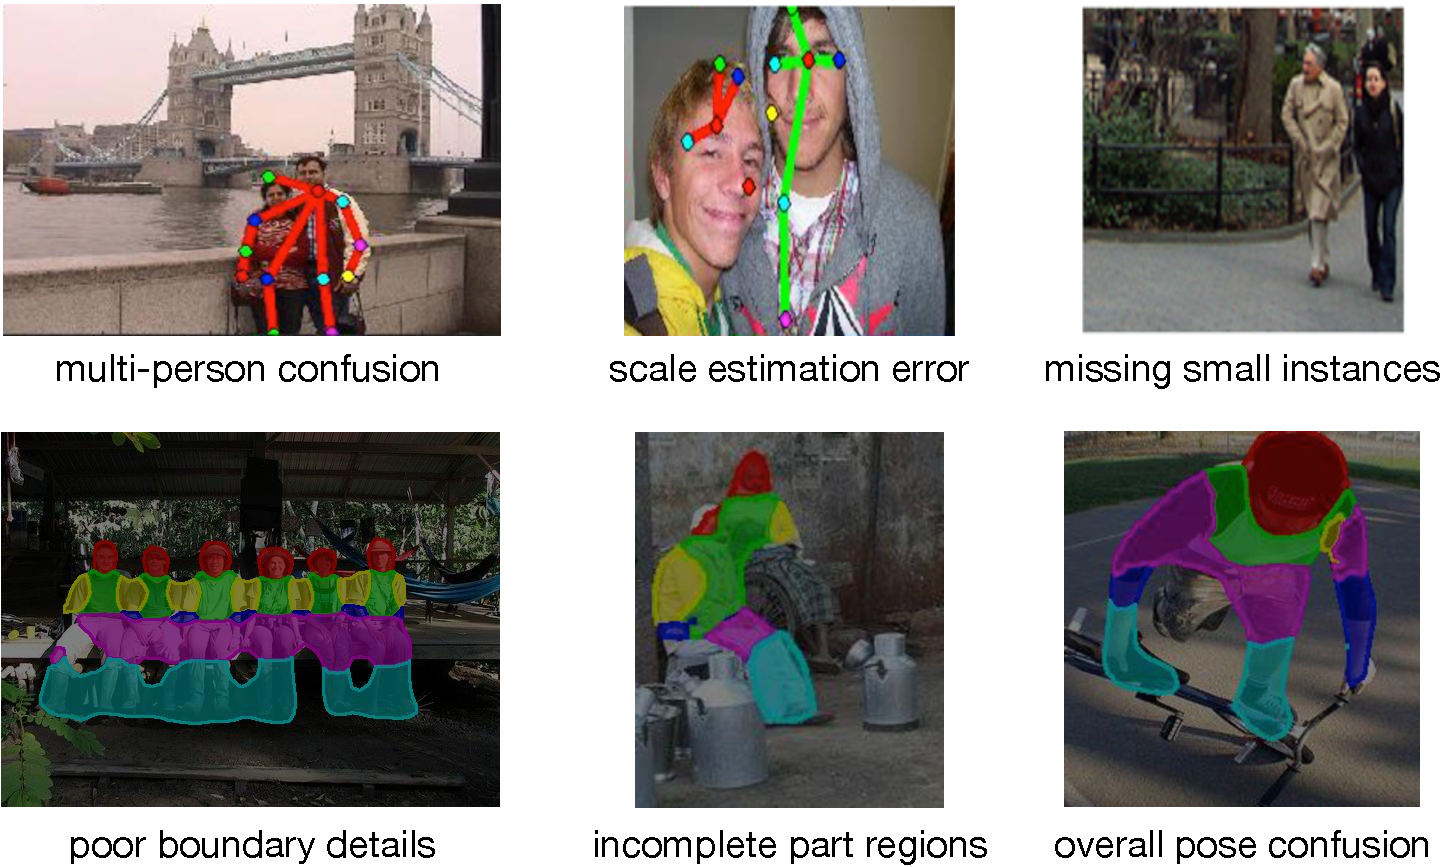
\includegraphics[width=1.0\linewidth]{figs/intro_hard.pdf}
\caption{Challenges for current human pose estimation algorithms (top row) and semantic part segmentation algorithms (bottom row) in natural multi-person scenes.}
\label{fig:challenge}
\end{figure}

\begin{figure*}
\begin{center}
 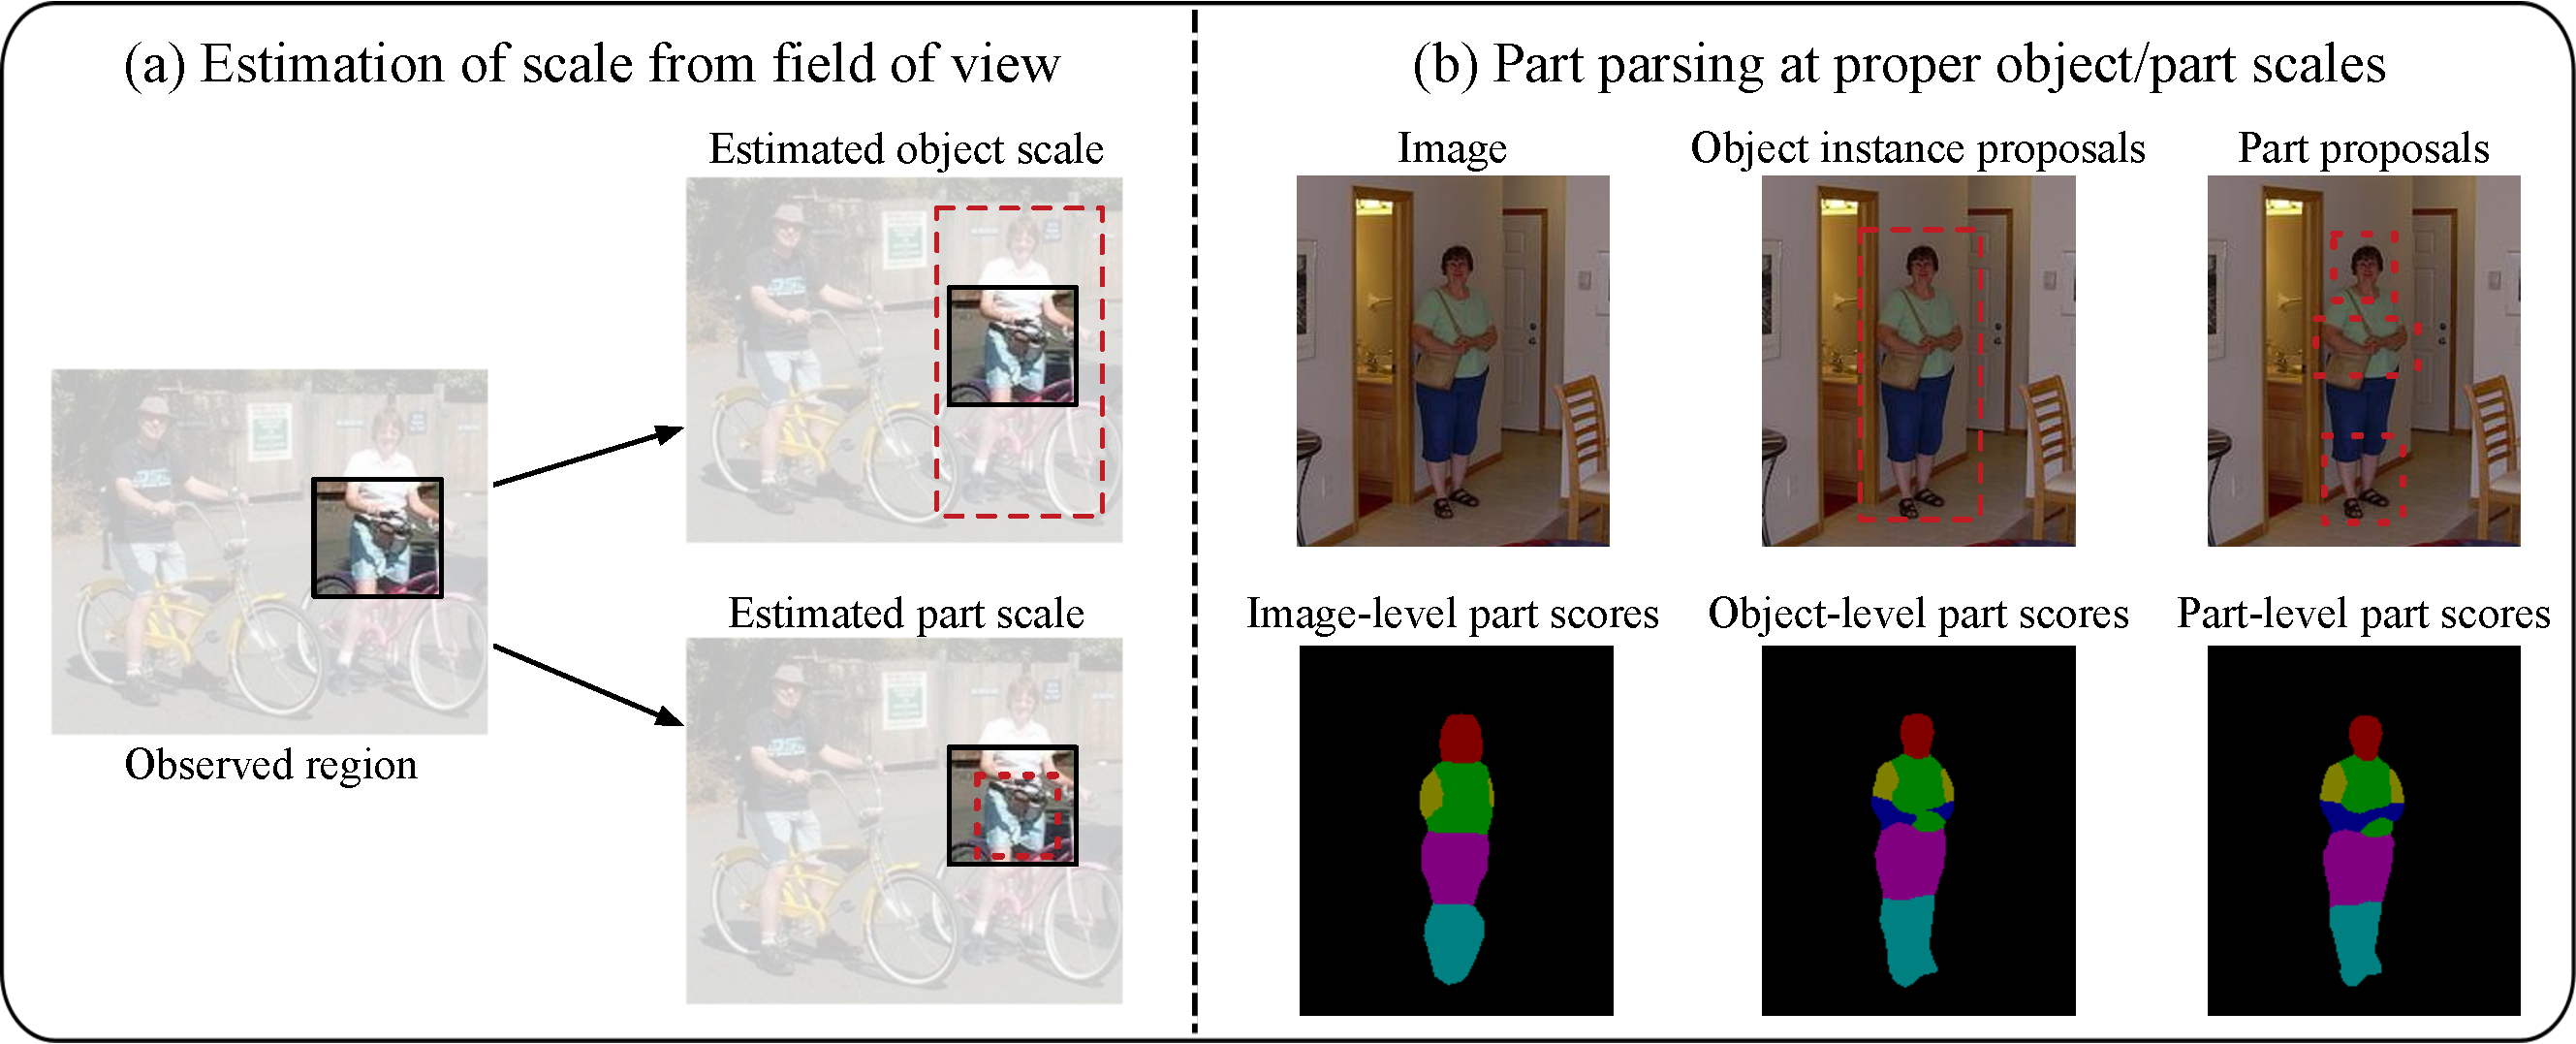
\includegraphics[width=0.8\textwidth]{figs/intuition_eccv.pdf}
\end{center}
\caption{Intuition of our hierarchical auto-zoom model (HAZN), which handles the large variation of object and part scale in natural multi-person scenes. (a) The scale
and location of an object and its parts (the red dashed boxes) can be estimated
from the observed field of view (the black solid box) of a neural network. (b)
Part segmentation can be more accurate by using proper object and part scales. In the top row, we show our estimated object and part scales. In the bottom row,
our part segmentation results gradually become better by increasingly utilizing the
estimated object and part scales.}
\label{fig:motivation_eccv}
\end{figure*}

% Difficulty of both tasks. Current methods and their shortcomings.
Currently, both semantic part segmentation and pose estimation face unsolved challenges in natural multi-person scenes (see Fig.~\ref{fig:challenge}).
Traditional semantic part segmentation methods~\cite{bo2011shape,eslami2012generative,yamaguchi2012parsing,dong2013deformable,zhu2011max} usually generate part segment proposals first and then use graphical models to select and assemble the part segment proposals into human instances. These methods are often time-consuming and only work well in constrained scenes, which pre-suppose known scale, fairly accurate localization, clear appearances, and/or relatively simple poses. Recently, dramatic progress has been made in semantic part segmentation due to the advent of fully convolutional neural networks (FCNs)~\cite{long2015fully} and the availability of object part annotations in large-scale datasets like PASCAL~\cite{chen2014detect}. These FCN-based methods~\cite{hariharan2015hypercolumns,wang2015joint,chen2016deeplab} usually compute pixel-wise part labels directly in a simple and fast way, and then optionally refine the labels by a graphical model such as the dense CRF~\cite{krahenbuhl2011efficient}. Although these FCN-based methods work well generally, they still suffer from the following two problems when handling natural multi-person scenes. They can make mistakes (e.g. missing small instances, producing poor boundary details or incomplete part regions, etc.) on small scale or extra large scale human instances for short of an effective mechanism to adapt to the size of the object instance. They also tend to produce erroneous predictions when the human instance is in an unusual pose or the appearance cues are weak, due to lack of object-level shape prior to regularize the part segments.

Similar to the trend of semantic part segmentation, traditional pose estimation approaches adopt graphical models to combine spatial constraints with local observations of joints, based on low-level features, like color intensities, HOG~\cite{dalal2005histograms}, shape-context~\cite{belongie2001shape}, and so on. Recent strategies rely on deep-learned joint detectors, and use a carefully designed graphical model to select and assemble joints into valid pose
configurations. Traditional approaches suffer from limited feature representation power and can only work in simple datasets with small pose and scale variation. Recent deep-based approaches have much better invariance to pose/scale variation, but their localization of joints is still inaccurate (e.g. joints are sometimes outside the human body) and they still struggle in multi-person overlapping scenes.

% Two main models in our framework.
In this paper, we present a scale-aware and pose-guided part segmentation framework that effectively improves human semantic part segmentation in natural images with large pose/scale variation. The framework mainly contains two novel models: (1) a hierarchical auto-zoom model (HAZN) that handles the large scale variation of human instances and human parts; (2) a joint prediction model that combines pose estimation and semantic part segmentation together, letting the two tasks benefit each other. Here we give a brief introduction to the two proposed models.

% Intuition of HAZN
The hierarchical ``auto-zoom" model (HAZN) model is a FCN-based model performing object/part scale estimation and part segmentation at the same time, adapting to the size of objects and parts. It's partially motivated by the proposal-free end-to-end detection strategies~\cite{huang2015densebox,liang2015proposal,ren2015faster,redmon2016you}. To get some intuition of this approach, observe in Fig.~\ref{fig:motivation_eccv}(a), that the scale and location of a target object, and of its corresponding
parts, can be estimated accurately from the field-of-view (FOV) window
by applying a deep neural network. Using estimated object and part scales, the semantic part segmentation results can become better and better, see Fig.~\ref{fig:motivation_eccv}(b). Please refer to Sec.~\ref{sec:hazn} for a detailed explanation of the HAZN model. 

\begin{figure}
 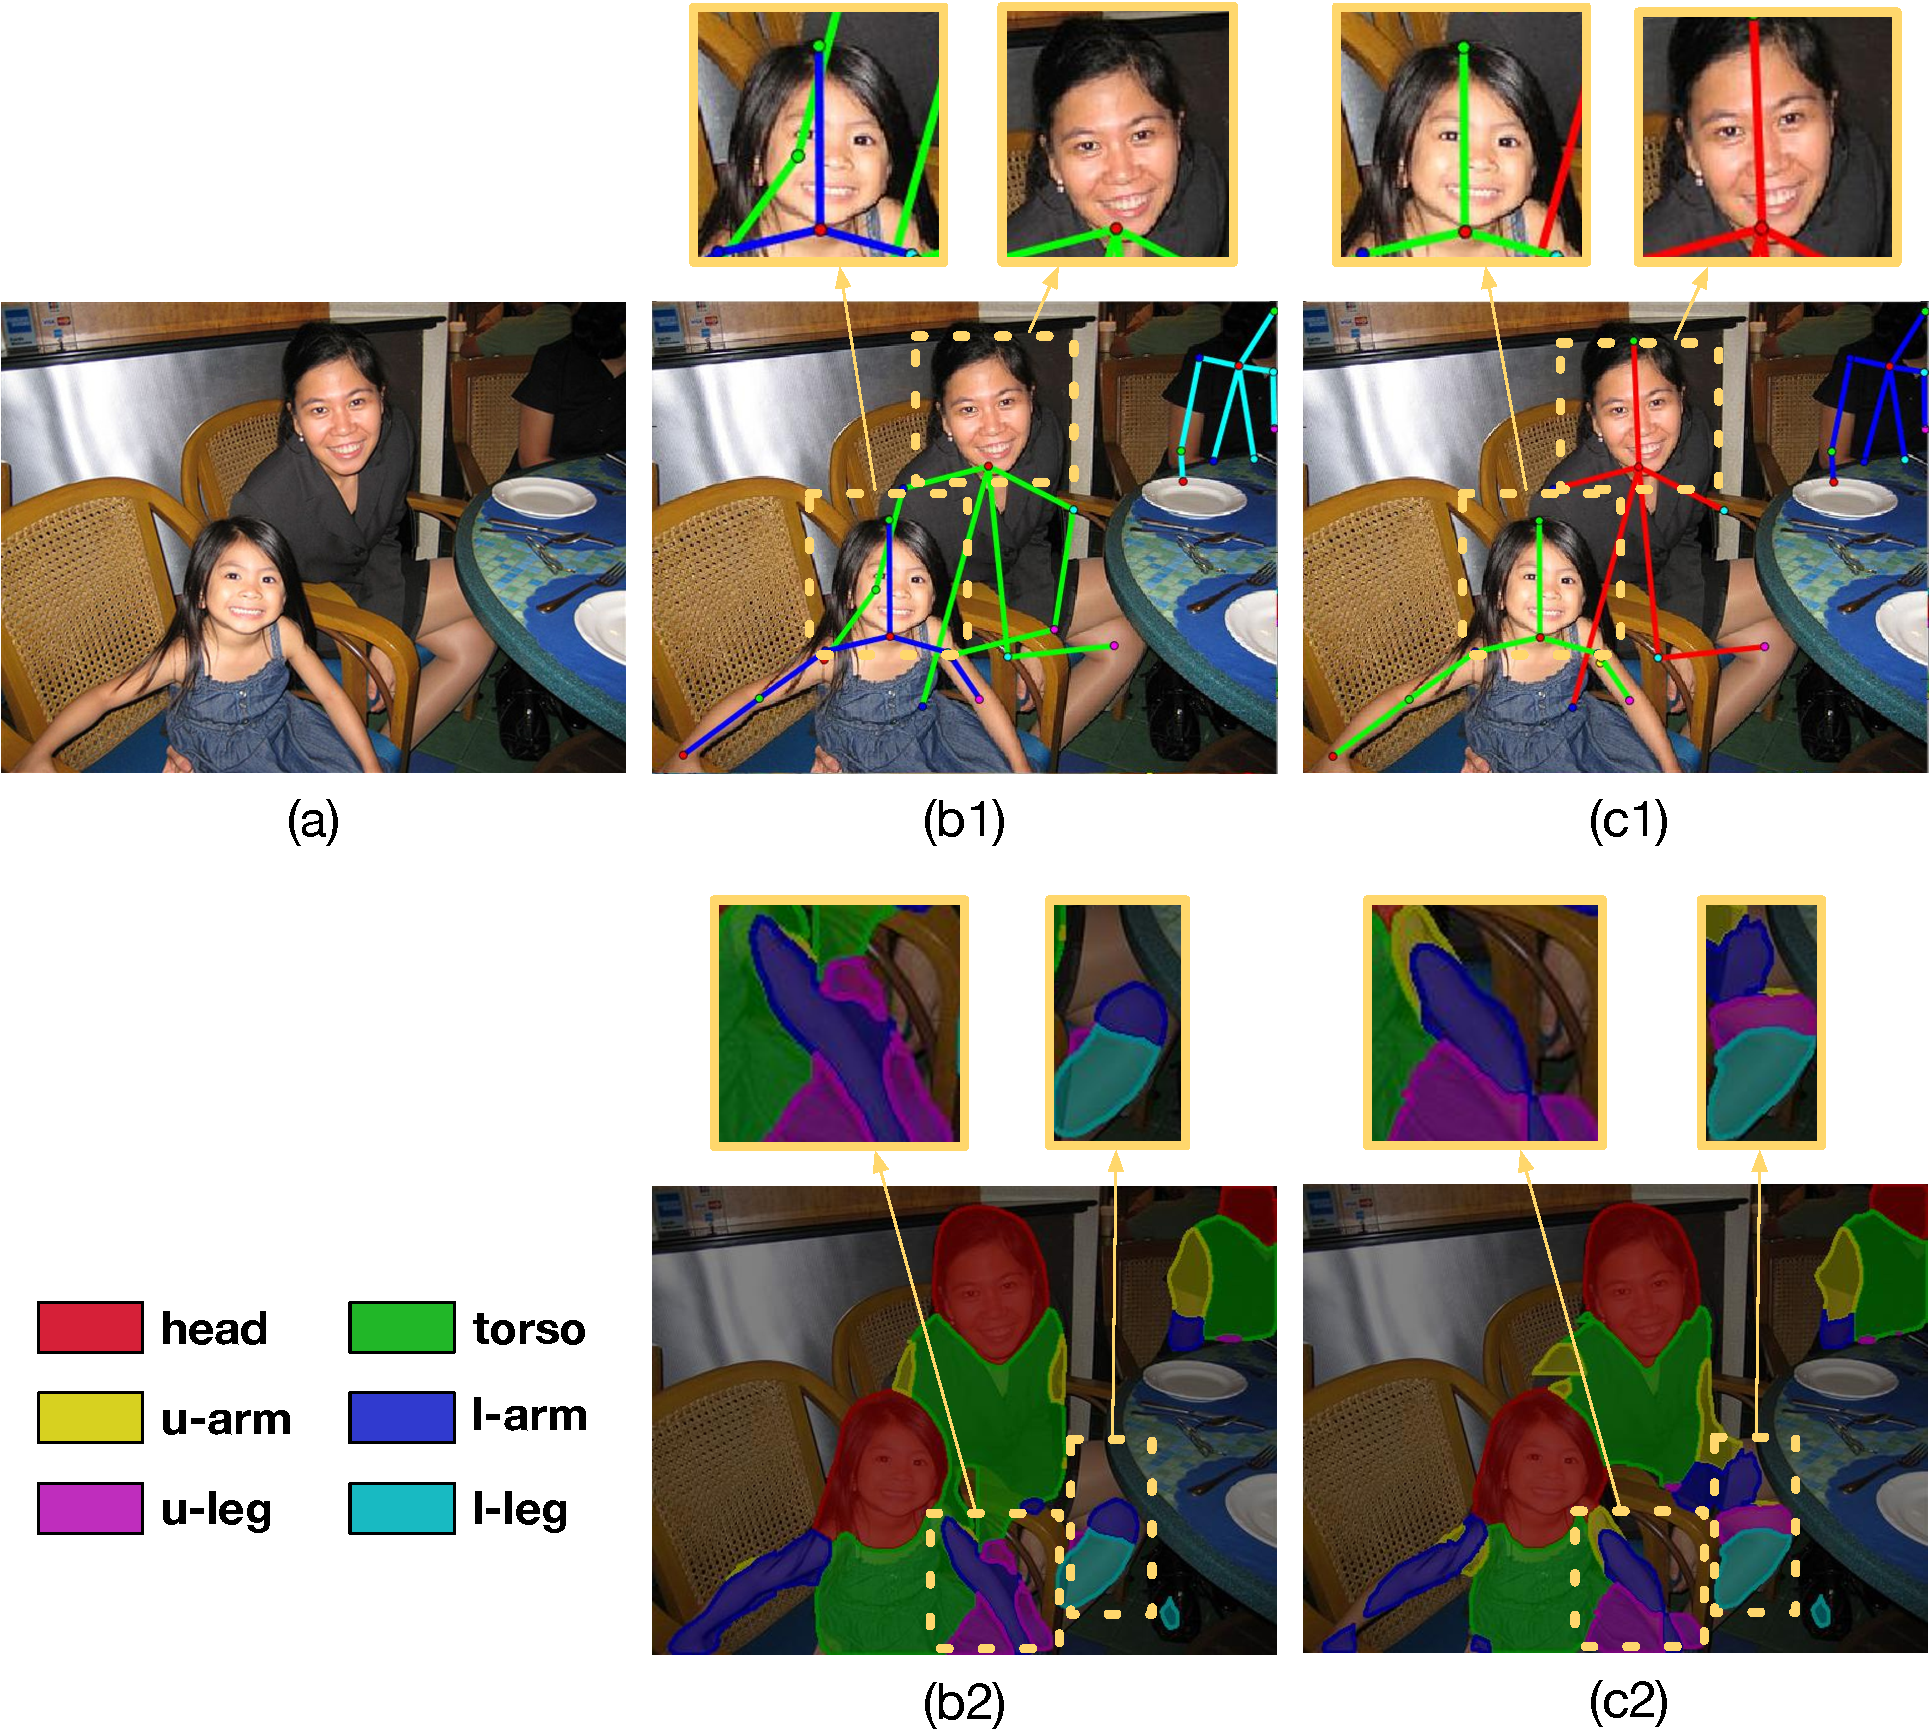
\includegraphics[width=1.0\linewidth]{figs/intuition_cvpr.pdf}
\caption{Joint human pose estimation and semantic part segmentation improve both tasks. (a) input image. (b) pose estimation and semantic part segmentation results before joint inference. (c) pose estimation and semantic part segmentation results after joint inference. Note that comparing (b1) and (c1), our result recovers the missing forehead joint and corrects the location error of right elbow and right wrist for the woman on the right. Comparing (b2) and (c2), our result gives more accurate details of lower arms and upper legs than (b2) for both people.}
\label{fig:motivation_cvpr}
\end{figure}

% Intuition of joint prediction model.
The joint prediction model is also a FCN-based framework aiming to solve the pose estimation task and the semantic part segmentation task jointly, in which the estimated pose provides object-level shape prior to regularize part segments (e.g. helping part segments align with human instances over the details of arms and legs where appearance cues are missing) while the part-level segments constrain the variation of pose locations (e.g. helping pose joints locate within their corresponding part segments). As shown in Fig.~\ref{fig:motivation_cvpr}, by taking advantage of the complementary property between pose estimation and semantic part segmentation, this joint prediction model produces better results on both tasks. See Sec.~\ref{sec:pose_and_seg} for detailed introduction of the model.

% Evaluation dataset and experiments.
In this paper, we address the task of human semantic part segmentation in ``the wild" where there are large variations in scale, pose, location, and occlusion. This motivates us to work with PASCAL images~\cite{everingham2014pascal} because these were chosen for studying multiple visual tasks, do not suffer from dataset design bias~\cite{li2014secrets}, and include large variations of objects, particularly of scale and pose. Hence human semantic part segmentation in PASCAL is considerably more difficult than in datasets, such as Fashionista~\cite{yamaguchi2012parsing}, that were constructed solely to evaluate human parsing. 

We illustrate our approach by extensive experiments on PASCAL-Person-Part dataset~\cite{chen2014detect}, which contains detailed part annotations for every person in a subset of PASCAL VOC 2010. We further augment this dataset with 14 pose joint locations through manual labeling to evaluate our joint prediction model. Our experiments show that our approach outperforms previous state-of-the-art methods for both semantic part segmentation and pose estimation tasks. We are particularly good at recovering small human parts, giving clearer details of arms and legs, and correcting local confusions of people.

\section{Related Works}
As human semantic part segmentation and human pose estimation are two fundamental topics in computer vision, many graphical models on the two topics have been proposed during the past thirty years. With the advent of powerful deep learning techniques, some models start to use deep-learned features, or even perform the whole task within a deep neural network. Recently, there are also works that combine pose estimation and segmentation in graphical models. In this section, we give an overall review of previous literature in these aspects.

\subsection{Human Semantic Part Segmentation}
Traditional methods on human semantic part segmentation fall into two major categories.
One type of methods first generate region/segment proposals for each semantic part, then select and assemble the region proposals by a graphical model.
Bo et al.~\cite{bo2011shape} generate region proposals by UCM segmentation~\cite{arbelaez2009contours}, rank the region proposals using shape and appearance features, and assemble the proposals with simple geometric constraints.
Dong et al.~\cite{dong2013deformable} get region proposals by UCM and CPMC~\cite{carreira2012cpmc}, extract a rich set of appearance features for each region proposal encoded by Fisher Kernel and second-order pooling, and assemble the region proposals with a dedicated And-Or graph (AOG).
The other type of methods treat semantic part segmentation as scene parsing, adopting pixel-wise conditional random fields (CRFs) to infer the pixel-wise part labels.
Yamaguchi et al.~\cite{yamaguchi2012parsing} build a CRF based on super-pixels and try to classify each super-pixel into one of the semantic part types.
They learn unary part classifiers for super-pixels based on traditional features, and use the output scores as unary terms in the CRF.
For the pairwise terms, they train logistic regression models to predict whether two neighboring pixels should have the same label, and also learn a consistency prior between each part type pair from the training data.
These traditional methods perform well on simple images, but struggle in natural images with large pose/scale variations.

Over the past few years, deep convolutional neural networks (DCNNs)~\cite{lecun1998gradient} have pushed the performance to new heights in many computer vision tasks such as image classification and object detection. DCNNs have also been applied to semantic object segmentation in the wild~\cite{chen2016deeplab,dai2015boxsup,papandreou2015weakly}, showing that DCNNs can also be applied to segment object parts in the wild.
Some extract deep-learned features for region proposals, and assemble the region proposals using a graphical model based on those features~\cite{xia2016pose}.
Some use fully convolutional networks (FCNs)~\cite{long2015fully} to output pixel-wise part labels directly, tailed by an optional CRF to smooth the part labels~\cite{long2015fully,chen2016deeplab,wang2015joint}. Graphical models with DCNN features perform well on relatively simple datasets and give good details of parts, but they struggle in complex natural datasets with large pose/scale variation. FCN-type approaches handle pose variation better, but they still suffer from large scale variation (e.g. missing parts or giving coarse part boundary details), and can produce local confusion errors (e.g. labeling arm regions as legs, labeling background regions as arms, etc.) if the person is in a non-typical pose, or when there are some other object/person nearby with similar appearance.

Recently, several works explore object-level context to produce better part segmentation results.
Hariharan et al.~\cite{hariharan2015hypercolumns} perform object detection, object segmentation and part segmentation sequentially, in which the object is first localized by a RCNN~\cite{girshick2014rich}, then the object (in the form of a bounding box) is segmented by a FCN to produce an object mask, and finally part segmentation is performed by partitioning the mask. The process has two potential drawbacks: (1) it is complex to train all components of the model; (2) the error from object masks, e.g. local confusion and inaccurate edges, propagates to the part segments.
Our hierarchical auto-zoom net model (HAZN) follows this general coarse-to-fine strategy, but is more unified and more importantly, we do not make premature decisions.
Wang et al.~\cite{wang2015joint} employ a two-stream FCN to jointly infer object and part segmentations for animals, where the part stream was performed to discover part-level details and the object stream was performed to find object-level context.
Although this work proves the usefulness of object-level context, it only uses a single-scale network for both object and part score prediction, where small-scale objects might be missed at the beginning and the scale variation of parts still remains unsolved.

Some other recent works try to handle the scale issue within a DCNN structure.
They commonly use multi-scale features from intermediate layers, and perform late fusion on them~\cite{long2015fully,hariharan2015hypercolumns,chen2016deeplab} in order to achieve scale invariance. Chen et al.~\cite{chen2016attention} propose a scale attention model, which learns pixel-wise weights for merging the outputs from three fixed scales.
These approaches, though developed on powerful DCNNs, are all limited by the number of scales they can select and the possibility that the scales they select may not cover a proper one. Our HAZN model avoids the scale selection error by directly regressing the bounding boxes for objects/parts and zooming the regions into proper scales.
In addition, this mechanism allows us to explore a broader range of scales, contributing a lot to the discovery of missing object instances and the accuracy of part boundaries.

\subsection{Human Pose Estimation}
Part-based graphical models are popular in human pose estimation due to the fact that human instances are highly articulated. 
Fischler and Elschlager~\cite{fischler1973representation} introduced the basic Pictorial Structural model (PS), a tree model with local part scores and kinematic pairwise terms.
However, exact inference of PS on dense pixels was too time consuming at that time. Fast inference on PS was made possible by Felzenszwalb and Huttenlocher~\cite{felzenszwalb2005pictorial}, who proposed efficient distance transform algorithms. 
Later, Andriluka~\cite{andriluka2009pictorial} improved Pictorial Structures by learning stronger part filters using Adaboost classifiers built on shape-context features of each part. Traditional models like PS suffer from two disadvantages.
They are tree-structured models with traditional hand-crafted features, so they have limited representation power and can't handle large variations in pose and appearance.
Besides, the pairwise terms are just geometric priors between part pairs, not strong and not data-dependent.
To enhance the representation power of traditional models, multimodal compositional models are proposed. For example, Yang et al.~\cite{yang2011articulated} learn modes at the part level, consider compositional parts that connect to simple parts and model their geometric constraints;
Sapp et al.~\cite{sapp2013modec} treat the entire human body as a mixture of templates;
Zhu et al.~\cite{zhu2008max} and RothRock et al.~\cite{rothrock2013integrating} explore mixtures at middle-part level using an And-Or Graph (AOG).
 
With the growing popularity of deep learning, recent methods rely on strong joint detectors trained by DCNNs~\cite{chen2014articulated,tompson2015efficient}, and often use a simple graphical model (e.g. tree model, And-Or Graph) to select and assemble joints into a valid pose configuration.
These recent methods perform much better than traditional ones, but the localization of joints is still inaccurate (e.g. sometimes outside the human body) and they still struggle when there are multiple people overlapping each other.
Some other approaches discard graphical models by modeling the spatial dependencies of joints within DCNNs~\cite{toshev2014deeppose,carreira2016human,chu2016structured}. These approaches perform well on relatively simple datasets, but their ability to handle large pose variations in natural multi-person datasets is limited.
A very recent work, Deeper-Cut~\cite{insafutdinov2016deepercut}, addresses the multi-person issue explicitly, using integer linear programming to cluster joint candidates into multiple human instances and assign joint types to each joint candidate.
Deeper-Cut handles multi-person overlapping well, but is very time-consuming (4 minutes per image) and its performance on datasets with large scale variation is not fully satisfactory. Our joint prediction model improves in these aspects by introducing a segment-joint consistency term that yields better localization of flexible joints such as wrists and ankles, and an effective auto-zoom strategy that can deal with humans of different sizes.

\begin{figure*}
\begin{center}
 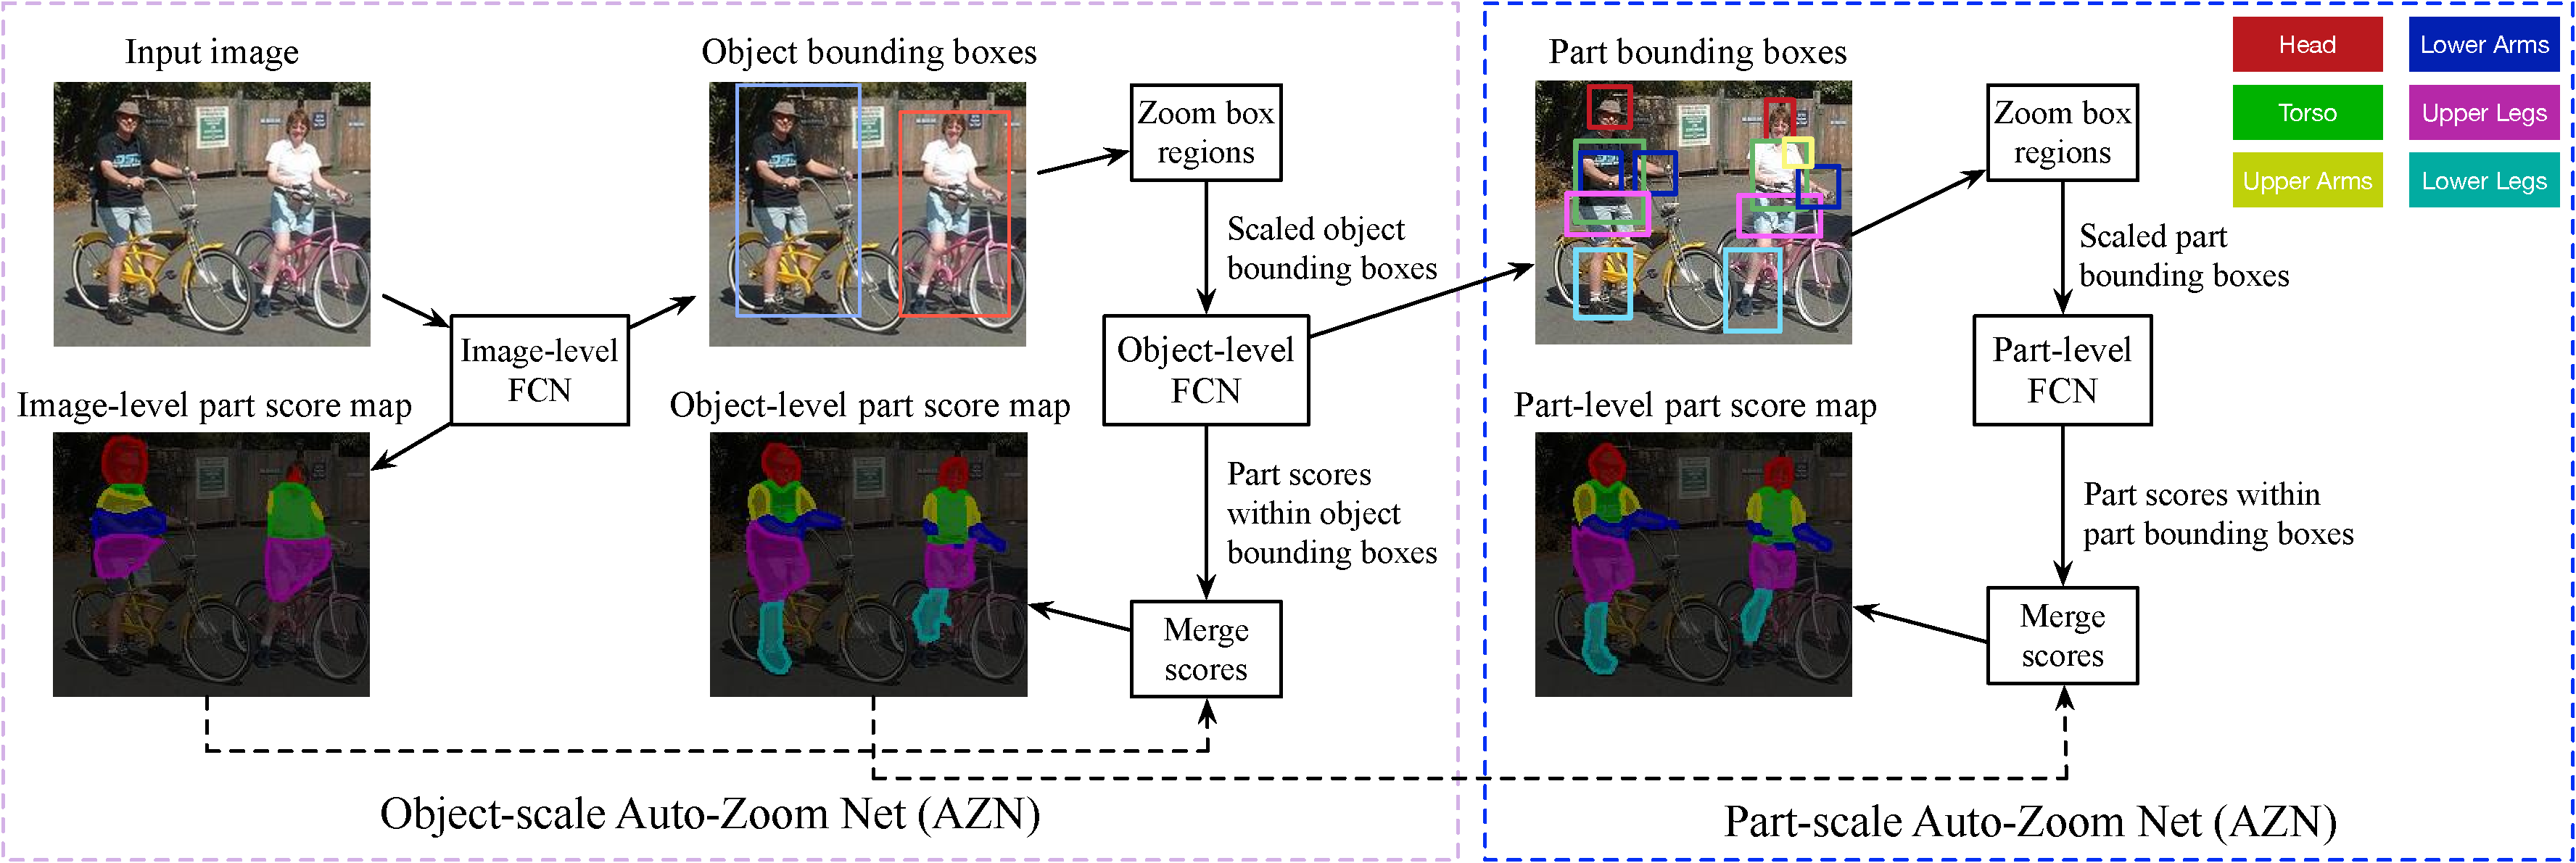
\includegraphics[width=1.0\textwidth]{figs/framework_eccv.pdf}
\end{center}
\caption{Testing framework of the Hierarchical Auto-Zoom Net (HAZN). We address object part parsing in a wild scene, adapting to the size of objects (object-scale AZN) and parts (part-scale AZN). The part scores are predicted and refined by three FCNs, over three levels of granularity, i.e. image-level, object-level, and part-level. At each level, the FCN outputs the part score map for the current level, and estimates the locations and scales for next level. The details of parts are gradually discovered and improved along the proposed auto-zoom process (i.e. location/scale estimation, region zooming, and part score re-estimation).}
\label{fig:framework_eccv}
\end{figure*}

\subsection{Joint Pose Estimation and Part Segmentation}
Recently, some researchers consider the correlation between pose estimation and segmentation. Yamaguchi et al.~\cite{yamaguchi2012parsing} perform human pose estimation and semantic part segmentation sequentially for clothes parsing, using a CRF with low-level features. Ladicky et al.~\cite{ladicky2013human} propose a principled formulation for joint pose estimation and part labeling under a CRF framework, using also low-level features. Dong et al.~\cite{dong2014towards} combine the two tasks with a manually designed And-Or graph. These methods demonstrate the complementary properties of the two tasks on relatively simple datasets, but they cannot deal with images with large pose variations or multi-person overlapping, mainly due to the less powerful features they use or the poor quality of their part region proposals. In contrast, our joint prediction model combines FCNs with graphical models, greatly boosting the representation power of models to handle large pose variation. We also introduce novel segment-joint consistency terms for both tasks, further improving the performance.

\section{Scale-Aware Part Segmentation Using Hierarchical Auto-Zoom Net}
\label{sec:hazn}
In this chapter, we will introduce a hierarchical method for object part segmentation that performs scale estimation
and object parsing jointly and is able to adapt its scale to objects and parts. Using fully convolutional nets (FCNs)~\cite{long2015fully} to predict
the scale and location of object instances and their corresponding parts (see Fig.~\ref{fig:motivation_eccv}(a)), the Hierarchical Auto-Zoom Net (HAZN)
parses the objects at three levels of granularity, namely image-level, object-level, and part-level, gradually giving clearer and better parsing results
(see Fig.~\ref{fig:motivation_eccv}(b)).

% Brief introduction of the inference process.
As shown in Fig.~\ref{fig:framework_eccv}, the HAZN sequentially combines two ``Auto-Zoom Nets" (AZNs), each of which predicts the locations and scales for objects (the first AZN) or parts (the second AZN), properly zooms (resizes) the predicted image regions, and refines the object parsing result for those image regions. The HAZN uses three fully convolutional neural networks (FCNs)~\cite{long2015fully} that share the same structure. The first FCN acts directly on the image to estimate a finite set of possible locations and sizes of objects (e.g. bounding boxes) with confidence scores, together with a part score map of the image. The part score map (in the bottom left of Fig.~\ref{fig:motivation_eccv}(b)) is similar to that proposed by previous deep-learned methods. The object bounding boxes are scaled to a fixed size by zooming in or zooming out (as applicable) and the image and part score maps within the boxes are also scaled (e.g. by bilinear interpolation for zooming in or downsampling for zooming out). Then the second FCN is applied to the scaled object bounding boxes to make proposals (bounding boxes) for the positions and sizes of the parts, with confidence values, and to re-estimate the part scores within the object bounding boxes. This yields improved part scores, see the bottom-middle score map of Fig.~\ref{fig:motivation_eccv}(b). We then apply the third FCN to the scaled part bounding boxes to produce new estimates of the part scores and to combine all of them (for different object and part bounding boxes) to output final part scores, see the bottom right of Fig.~\ref{fig:motivation_eccv}(b), which are our parse of the object. This strategy is modified slightly so that, for example, we scale humans differently depending on whether we have detected a complete human or only the upper part of a human, which can be determined automatically from the part score map.

We illustrate the effectiveness of our ``auto-zoom'' approach by extensive experiments for parsing humans on the PASCAL-Person-Part dataset~\cite{chen2014detect} and for parsing animals on a horse-cow dataset~\cite{wang2015semantic}. These datasets are challenging because they have large variations in scale, pose, and location of the objects. We now briefly comment on the advantages of our approach for dealing with scale and how it differs from traditional methods. Previous methods mainly select a fixed set of scales in advance and then perform fusion on the outputs of a deep net at different layers. Computational requirements mean that the number of scales must be small and it is impractical (due to memory limitations) to use very fine scales. Our approach is considerably more flexible because we adaptively estimate scales at different regions in the image which allows us to search over a large range of scales. In particular, we can use very fine scales because we will probably only need to do this within small image regions. For example, our largest zooming ratio is 2.5 (at part level) on PASCAL while that number is 1.5 if we have to zoom the whole image. This is a big advantage when trying to detect small parts, such as the tail of a cow, as is shown by the experiments. In short, the adaptiveness of our approach and the way it combines scale estimation with parsing give novel computational advantages.

\subsection{The Model}
As demonstrated in Fig.~\ref{fig:framework_eccv}, our Hierarchical Auto-Zoom Net (HAZN) has three levels of granularity for tackling scale variation in object part segmentation,
i.e. image-level, object-level, and part-level. At each level, a fully convolutional neural network (FCN) is used to perform scale/location estimation and part parsing simultaneously. The three levels of FCNs are all built on the same network structure, a modified FCN proposed by Chen et al.~\cite{chen2016deeplab}, namely DeepLab-LargeFOV. This network structure is one of the most effective FCNs in segmentation, so we also treat it as our baseline for final performance comparison.

To handle scale variation in objects and parts, the HAZN concatenates two Auto-Zoom Nets (AZNs), namely object-scale AZN and part-scale AZN, into a unified network. The object-scale AZN refines the image-level part score map with object bounding box proposals while the part-scale AZN further refines the object-level part score map with part bounding box proposals. Each AZN employs an auto-zoom process: first estimates the region of interest (ROI), then properly resizes the predicted regions, and finally refine the part scores within the resized regions.

\subsubsection{Object-Scale Auto-Zoom Net (AZN)}
\label{subsubsec:AZN}
For the task of object part segmentation, we are provided with $n$ training examples $\{\ve{I}_i, \ve{L}_i\}_{i=1}^{n}$, where $\ve{I}$ is the given image and $\ve{L}$ is the supervision information that provides discrete semantic labels of interest. Our target is to learn the posterior distribution $P(l_j | \ve{I},j)$ for each pixel j of an image $\ve{I}$. This distribution is approximated by our object-scale AZN, as shown in Fig.~\ref{fig:prob_model_eccv}.

\begin{figure*}
\begin{center}
   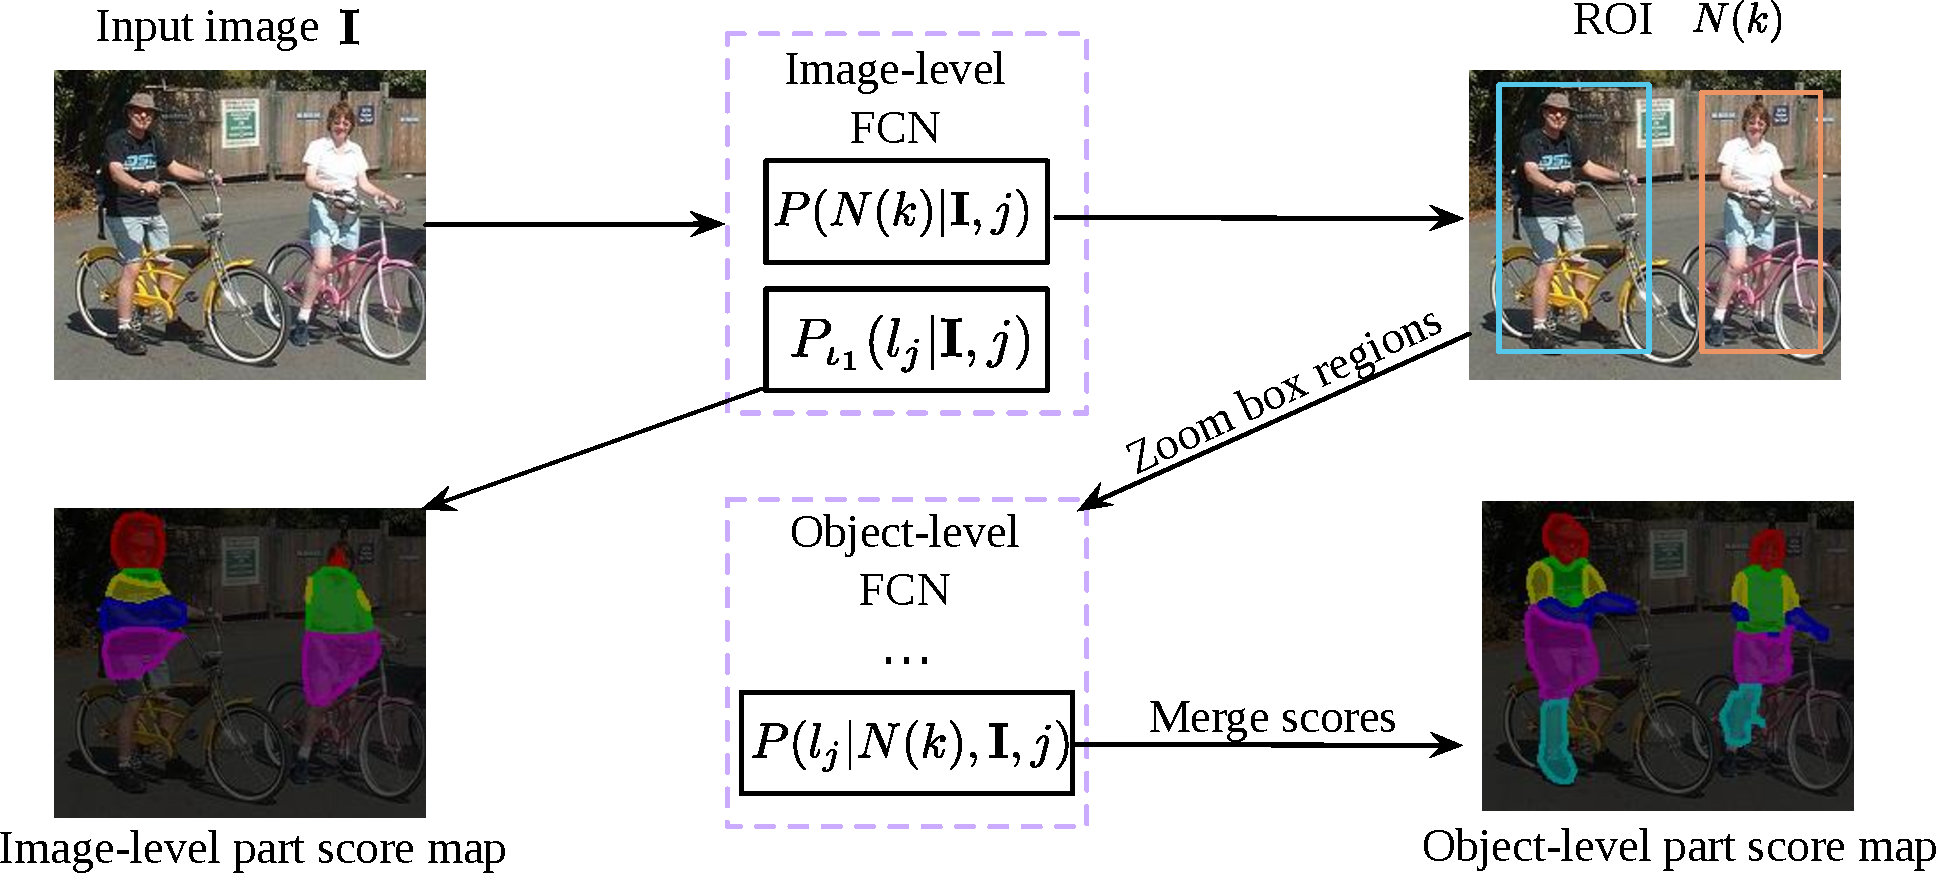
\includegraphics[width=0.8\linewidth]{figs/prob_model_eccv.pdf}
\end{center}
 \caption{Object-scale auto-zoom model from a probabilistic view, which predicts ROI region $N(k)$ at object-scale, and then refines part scores based on the properly zoomed region $N(k)$. Details are in Sec.~\ref{subsubsec:AZN}.}
\label{fig:prob_model_eccv}
\end{figure*}

% The part parsing network and the scale estimation network
We first use the image-level FCN (see Fig.~\ref{fig:framework_eccv}) to produce the image-level part score map $P_{\iota_1}(l_j | \ve{I},j)$, which gives comparable performance to our baseline method (DeepLab-LargeFOV). This is a normal \emph{\textbf{part parsing network}} that uses the original image as input and outputs the pixel-wise part score map. Our object-scale AZN aims to refine this part score map with consideration of object instance scales. To do so, we add a second component to the image-level FCN, performing regression to estimate the size and location of an object bounding box (or ROI) for each pixel, together with a confidence map indicating the likelihood that the box is an object. This component is called a \emph{\textbf{scale estimation network}} (\textbf{SEN}), which shares the first few layers with the part parsing network in the image-level FCN. In math, the SEN corresponds to a probabilistic model $P(b_j | \ve{I}, j)$, where $b_j$ is the estimated bounding box for pixel $j$, and $P(b_j|...)$ is the confidence score of $b_j$.

% NMS and region zooming
After getting $\{b_j |\forall j\in\ve{I}\}$, we threshold the confidence map and perform non-maximum suppresion to yield a finite set of object ROIs (typically 5-10 per image, with some overlap): $\{b_k | k \in \ve{I}\}$. Each $b_k$ is associated with a confidence score $P(b_k)$. As shown in Fig.~\ref{fig:framework_eccv}, a \textbf{region zooming} operation is then performed on each $b_k$, resizing $b_k$ to a standard-sized ROI $N(k)$. Specifically, this zooming operation computes a zooming ratio $f(b_k, L^{b_k}_p)$ for bounding box $b_k$, based on the bounding box $b_k$ and the computed image-level part labels $L^{b_k}_p$ within the bounding box, and then enlarges or shrinks the image within the bounding box by the zooming ratio. We will discuss $f()$ in detail in Sec.~\ref{subsec:exp}.

% Re-predict the part labels
Now we have a set of zoomed ROI proposals $\{N(k)|k\in\ve{I}\}$, each $N(k)$ associated with score $P(b_k)$. We learn another probabilistic model $P(l_j | N(k), \ve{I}, j)$, which re-estimates the part label for each pixel $j$ within the zoomed ROI $N(k)$. This probabilistic model corresponds to the part parsing network in the object-level FCN (see Fig.~\ref{fig:framework_eccv}), which takes as input the zoomed object bounding boxes and outputs the part scores within those object bounding boxes.

% Score merging
The new part scores for the zoomed ROIs need to be merged to produce the object-level part score map for the whole image. Since there may be multiple ROIs that cover a pixel $j$, we define the neighbouring region set for pixel j as $\hua{Q}(j)=\{N(k) | j \in N(k), k \in \ve{I}\}$. Under this definition of $\hua{Q}(j)$, the \textbf{score merging} process can be expressed as Equ.~\ref{eqn:AZN}, which essentially computes the weighted sum of part scores for pixel $j$, from the zoomed ROIs that cover $j$. For a pixel that is not covered by any zoomed ROI, we simply use its image-level part score as the current part score. Formally, the object-level part score $P_{\iota_2}(l_j|\ve{I}, j)$, is computed as, 
\begin{align}
P_{\iota_2}(l_j|\ve{I}, j) &= \sum\nolimits_{N(k) \in \hua{Q}(j)} P(l_j | N(k), \ve{I}, j) P(N(k) | \ve{I}, j);  \nonumber \\
P(N(k) | \ve{I}, j) &= P(b_k) / \textstyle{\sum_{k: N(k) \in \hua{Q}(j)} P(b_k)}
\label{eqn:AZN}
\end{align}

\subsubsection{Hierarchical Auto-Zoom Net (HAZN)}
The scale of object parts can also vary considerably even if the scale of the object is fixed. This leads to a hierarchical strategy with multiple stages,
called the Hierarchical Auto-Zoom Net (HAZN), which applies AZNs to images to find objects and then on objects to find parts, followed by a refinement stage.
As shown in Fig.~\ref{fig:framework_eccv}, we add the part-scale AZN to the end of the object-scale AZN.

We add a second component to the object-level FCN, i.e. the SEN network, to estimate the size and location of part bounding boxes,
together with confidence maps for every pixel within each zoomed object ROI. Again the confidence map is thresholded, and non-maximal suppresion is applied,
to yield a finite set of part ROIs (typically 5-30 per image, with some overlap). Each part ROI is zoomed to a fixed size.
Then, we re-estimate the part scores within each zoomed part ROI using the part parsing network in the part-level FCN.
The part parsing network is the only component of the part-level FCN, which takes the zoomed part ROI and the zoomed object-level part scores (within the part ROI) as inputs.
After getting the part scores within each zoomed Part ROI, the score merging process is the same as in the object-scale AZN.

It's easy to extend our HAZN model to include more AZNs at finer scale levels if we focus on smaller object parts such as human eyes.
If the HAZN contains $n$ AZNs, there are $n+1$ FCNs needed to be trained.
The $\iota$-th FCN learns $P_\iota(l_j | N(j)_{\iota-1}, ...)$ to refine the part scores based on the scale/location estimation results $P_{\iota-1}(N(j)_{\iota-1} | ...)$
and the part parsing results $P_{\iota-1}(l_j | N(j)_{\iota-1}, ...)$ from the previous level $\iota-1$.
At the same time, the $\iota$-th FCN also learns $P_\iota(N(j)_l | ...)$ to estimate the region of interest (ROI) for the next level $\iota+1$.

\subsubsection{Training and Testing Phases for Object-Scale AZN} 
\label{subsubsec:train_test}
In this section, we introduce the specific networks to learn our probalistic models. Specifically, we use a modern version of FCN, i.e. \textbf{DeepLab-LargeFOV}~\cite{chen2016deeplab}, as our basic network structure. DeepLab-LargeFOV is a stronger variant of DeepLab~\cite{chen2016deeplab}, which takes the raw image as input, and outputs dense feature maps. DeepLab-LargeFOV modifies the filter weights at the $fc_6$ layer so that its field-of-view is larger. We refer our readers to the original paper for details.

\begin{figure*}
\begin{center}
   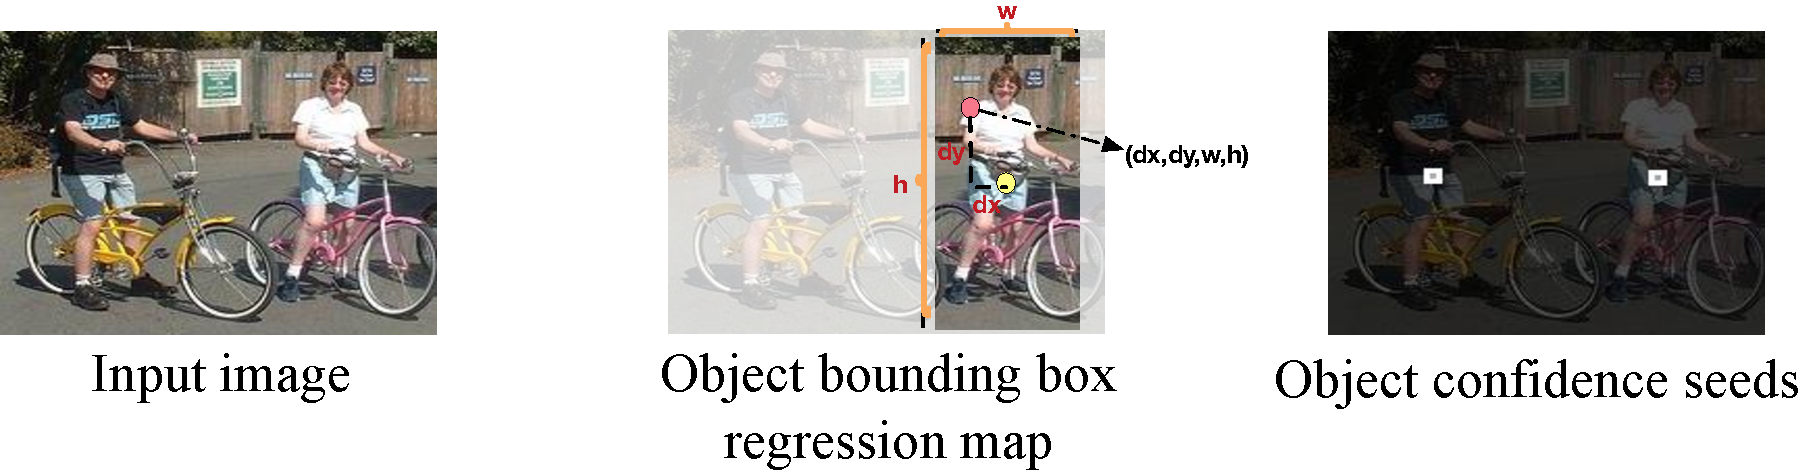
\includegraphics[width=0.8\linewidth]{figs/model_eccv.pdf}
\end{center}
\caption{Ground truth regression target for training the scale estimation network (SEN) in the image-level FCN. Details in Sec.~\ref{subsubsec:train_test}.}
\label{fig:train_sen}
\end{figure*}

\paragraph{\textbf{Training the SEN.}}
The scale estimation network (SEN) aims to regress the region of interest (ROI) for each pixel $j$ in the form of a bounding box, $b_j$.
Here we borrow the idea presented in the DenseBox~\cite{huang2015densebox} to do scale estimation, since it is simple and performing well enough for our task. 
In detail, at object level, the ROI of pixel $j$ corresponds to the object instance box that pixel $j$ belongs to. For training the SEN,
two output label maps are needed as visualized in Fig.~\ref{fig:train_sen}. The first one is the bounding box regression map $\ve{L}_{b}$,
which is a four-channel output for each pixel $j$ to represent its ROI $b_j$: $\ve{l}_{bj}=\{dx_j, dy_j, w_j, h_j\}$.
Here $(dx_j, dy_j)$ is the relative position from pixel $j$ to the center of $b_j$; $h_j$ and $w_j$ are the height and width of $b_j$.
We then re-scale the outputs by dividing them with $400$. 
The other target output map is a binary confidence seed map $\ve{L}_{c}$, in which $\ve{l}_{cj}\in\{0,1\}$ is the ROI selection indicator at pixel $j$.
It indicates the preferred pixels for us to use for ROI prediction, which helps the algorithm prevent many false positives.
In practice, we choose the central pixels of each object instance as the confidence seeds,
which tend to predict the object bounding boxes more accurately than those pixels at the boundary of an object instance region. 

Given the ground-truth label map of object part parsing, we can easily derive the training examples for the SEN:
$\hua{H} = \{\ve{I}_i, \ve{L}_{bi}, \ve{L}_{ci}\}_{i=1}^{n}$, where $n$ is the number of training instances.
We minimize the negative log likelihood to learn the weights $\ve{W}$ for the SEN, and the loss $l_{SEN}$ is defined in Equ.~\ref{eqn:loss_sen}.
\begin{align}
\label{eqn:loss_sen}
l_{SEN}(\hua{H}|\ve{W}) =& \frac{1}{n}\sum\nolimits_{i}(l_{b}(\ve{I}_i, \ve{L}_{bi} | \ve{W}) + \lambda l_{c}(\ve{I}_i, \ve{L}_{ci} | \ve{W})) \nonumber\\
l_{c}(\ve{I}, \ve{L}_{c}|\ve{W}) =& -\beta\sum\limits_{j:l_{cj}=1} \log P(l_{cj}^*=1|\ve{I}, \ve{W}) \nonumber \\
                                  & -(1-\beta)\sum\limits_{j:l_{cj}=0}\log P(l_{cj}^*=0|\ve{I}, \ve{W}) \\
l_{b}(\ve{I}, \ve{L}_{b}|\ve{W}) =& \frac{1}{|\ve{L}_{cj}^+|}\sum\nolimits_{j:l_{cj}=1}\|\ve{l}_{bj}-\ve{l}_{bj}^*\|^2 \nonumber
\end{align}
For the confidence seeds, we employ the balanced cross entropy loss, where $l_{cj}^*$ and $l_{cj}$ are the predicted value and ground truth value respectively. The probability is from a sigmoid function performing on the activation of the last layer of the CNN at pixel $j$.  $\beta$ is defined as the proportion of pixels with $l_{cj}=0$ in the image, which is used to balance the positive and negative instances. The loss for bounding box regression is the Euclidean distance over the confidence seed points, and $|\ve{L}_{cj}^+|$ is the number of pixels with $l_{cj}=1$.

\paragraph{\textbf{Testing the SEN.}}
For testing, the SEN outputs both the confidence score map $P(l_{cj}^*=1|\ve{I}, \ve{W})$ and a four-dimensional bounding box $\ve{l}_{bj}^*$ for each pixel $j$.
We regard a pixel $j$ with confidence score higher than $0.5$ to be reliable and output its bounding box $b_j = \ve{l}_{bj}^*$, associated with confidence score
$P(b_j) = P(l_{cj}^*=1|\ve{I}, \ve{W})$. We perform non-maximum suppression based on the confidence scores,
yielding several bounding boxes $\{\ve{b}_j | j=1,2,...\}$ as candidate ROIs with confidence scores $P(\ve{b}_j)$.
Each candidate ROI $b_j$ is then properly zoomed, becoming $N(j)$.

\paragraph{\textbf{Training the part parsing network.}}
The training of the part parsing network is standard. For the object-level FCN, the part parsing network is trained based on all the the zoomed image regions (ROIs),
with the ground-truth part label maps $\hua{H_p} = \{\ve{L}_{pi}\}_{i=1}^{n}$ within the zoomed ROIs.
For the image-level FCN, the part parsing network is trained based on the original training images, and has the same structure as the scale estimation network (SEN) in the FCN.
Therefore, we merge the part parsing network with the SEN, yielding the image-level FCN with loss defined in Equ.~\ref{eqn:AZN_loss}.
Here, $l_{p}(\ve{I}, \ve{L}_{p})$ is the commonly used multinomial logistic regression loss for classification.
\begin{align}
\label{eqn:AZN_loss}
l_{AZN}(\hua{H},\hua{H_p}|\ve{W}) =\frac{1}{n}\sum\nolimits_il_{p}(\ve{I}_i, \ve{L}_{pi}) + l_{SEN}(\hua{H}|\ve{W})
\end{align}

\paragraph{\textbf{Testing the part parsing network.}}
For testing the object-scale AZN, we first run the image-level FCN, yielding part score maps at the image level and bounding boxes for the object level.
Then we zoom onto the bounding boxes and parse these regions based on the object-level FCN model, yielding part score maps at the object level.
By merging the part score maps from the two levels, we get better parsing results for the whole image.

\subsection{Experiments}
\label{subsec:exp}

\subsubsection{Implementation Details}
\paragraph{\textbf{Selection of confidence seeds.}}
To train the scale estimation network (SEN), we need to select confidence seeds for object instances or parts.
For human instances, we use the human instance masks provided by the PASCAL-Person-Part Dataset~\cite{chen2014detect} and
select the central $7\times7$ pixels within each instance mask as the confidence seeds. To get the confidence seeds for human parts,
we first compute connected part segments from the groundtruth part label map, and then also select the central $7\times7$ pixels within each part segment.
We present the details of our approach for humans because the extension to horses and cows is straightforward.

\paragraph{\textbf{Zooming ratio of ROIs.}}
The SEN networks in the FCNs provide a set of human/part bounding boxes (ROIs), $\{b_j | j\in \ve{I}\}$,
which are then zoomed to a proper human/part scale. The zooming ratio of $b_j$, $f(b_j, L^{b_j}_p)$,
is decided based on the size of $b_j$ and the previously computed part label map $L^{b_j}_p$ within $b_j$.
We use slightly different strategies to compute the zooming ratio at the human and part levels. 
For the part level, we simply resize the bounding box to a fixed size, i.e. $f_p(b_j) = s_t / max(w_j, h_j)$,
where $s_t = 255$ is the target size. Here $w_j$ and $h_j$ are the width and height of $b_j$. 
For the human level, we need to consider the frequently occurred truncation case when only the upper half of a human instance is visible. 
In practice, we use the image-level part label map $L^{b_j}_p$ within the box, and check the existence of legs to decide whether the full body is visible.
If the full body is visible, we use the same strategy as parts. Otherwise, we change the target size $s_t$ to $140$,
yielding relative smaller region than the full body visible case. We select the target size based on a validation set. 
Finally, we limit all zooming ratio $f_p(b_j)$ within the range $[0.4, 2.5]$ for both human and part bounding boxes to avoid artifacts from up or down sampling of images.

\subsubsection{Experimental Protocol}
\paragraph{\textbf{Dataset.}}
We conduct experiments on humans part segmentation using the PASCAL-Person-Part dataset~\cite{chen2014detect}, which is a subset from the PASCAL VOC 2010 dataset.
The dataset contains detailed part annotations for every person, e.g. head, torso, etc. We merge the annotations into six clases:
Head, Torso, Upper/Lower Arms and Upper/Lower Legs (plus one background class). 
We only use those images containing humans for training (1716 images in the training set) and testing (1817 images in the validation set),
the same as~\cite{chen2016attention}. Note that parsing humans in PASCAL is challenging because it has larger variations in scale and pose than other human parsing datasets. 
In addtion, we also perform parsing experiments on the horse-cow dataset~\cite{wang2015semantic}, which contains animal instances in a rough bounding box.
In this dataset, we keep the same experimental setting with~\cite{wang2015joint}.

\paragraph{\textbf{Training.}}
We train the FCNs using stochastic gradient descent with mini-batches. Each mini-batch contains 30 images.
The initial learning rate is 0.001 (0.01 for the final classifier layer) and is decreased by a factor of 0.1 after every 2000 iterations.
We set the momentum to be 0.9 and the weight decay to be 0.0005. The initialization model is a modified VGG-16 network pre-trained on ImageNet.
Fine-tuning our network on all the reported experiments takes about 30 hours on a NVIDIA Tesla K40 GPU.
After training, the average inference time for one PASCAL image is 1.3 s/image.

\paragraph{\textbf{Evaluation metric.}}
The object part segmentation results are evaluated in terms of mean IOU (mIOU).
It is computed as the pixel intersection-over-union (IOU) averaged across classes~\cite{everingham2014pascal},
which is also used recently to evaluate parts~\cite{wang2015joint,chen2016attention}.
We also evaluate the part segmentation performance w.r.t. each object instance in terms of $AP^r_{part}$ as defined in~\cite{hariharan2015hypercolumns}.

\paragraph{\textbf{Network architecture.}}
We use DeepLab-LargeFOV~\cite{chen2016deeplab} as building blocks for the FCNs in our Hierarchical Auto-Zoom Net (HAZN).
Recall that our HAZN consists of three FCNs working at different levels of granularity: image level, object level, and part level.
At each level, HAZN outputs part parsing scores, and estimats locations and scales for the next level of granularity (e.g. objects or parts).

\subsubsection{Experimental Results on Parsing Humans in the Wild}
\label{subsubsec:human_parsing_eccv}

\paragraph{\textbf{Comparison with state-of-the-arts.}}
As shown in Tab.~\ref{table:seg_eval_eccv}, we compare our full model (HAZN) with four baselines. The first baseline is DeepLab-LargeFOV~\cite{chen2016deeplab}.
The second one is DeepLab-LargeFOV-CRF, which adds a post-processing step to DeepLab-LargeFOV by means of a fully-connected Conditional Random Field (CRF)~\cite{krahenbuhl2011efficient}. CRFs are commonly used as postprocessing for object semantic segmentation to refine boundaries~\cite{chen2016deeplab}.
The third one is Multi-Scale Averaging, which feeds the DeepLab-LargeFOV model with images resized to three fixed scales (0.5, 1.0 and 1.5) and then
takes the average of the three part score maps to produce the final parsing result.
The fourth one is Multi-Scale Attention~\cite{chen2016attention}, a most recent work which uses a scale attention model to handle the scale variations in object part segmentation.
\begin{table}[!tb]
\centering
\setlength{\tabcolsep}{5pt}
\resizebox{1\columnwidth}{!}{
\begin{tabular}{l | c c c c c c c | c}
\toprule[0.2 em]
Method & head & torso & u-arms & l-arms & u-legs & l-legs & bg & Avg \\ \midrule \midrule
DeepLab-LargeFOV~\cite{chen2016deeplab} & 78.09 & 54.02 & 37.29 & 36.85 & 33.73 & 29.61 & 92.85 & 51.78 \\
DeepLab-LargeFOV-CRF & 80.13 & 55.56 & 36.43  & 38.72 & 35.50 & 30.82  & 93.52 & 52.95 \\
Multi-Scale Averaging & 79.89 & 57.40 & 40.57 & 41.14 & 37.66 & 34.31 & 93.43 & 54.91 \\
Multi-Scale Attention~\cite{chen2016attention} & \textbf{81.47} & 59.06 & 44.15 & 42.50 & 38.28 & 35.62 & 93.65 & 56.39 \\
\hline 
%DeepLab-LargeFOV-MSc & 79.43 & 55.01 & 39.03 & 39.95 & 35.44 & 32.28 & 93.14 & 53.47 \\
HAZN (no object scale) & 80.25 & 57.20 & 42.24 & 42.02 & 36.40 & 31.96 & 93.42 & 54.78 \\
HAZN (no part scale) & 79.83 & 59.72 & 43.84 & 40.84 & 40.49 & 37.23 & 93.55 & 56.50 \\
%Hierarchical Zooming (MSc + LargeFOV) & 80.66 & 58.73 &  42.60 & 42.65 & 39.01 & 34.36 & 93.55 & 55.94 \\
HAZN (full model) & 80.76 & \textbf{60.50} & \textbf{45.65} & \textbf{43.11} & \textbf{41.21} & \textbf{37.74} & \textbf{93.78} & \textbf{57.54} \\
\bottomrule[0.1 em]
\end{tabular}
}
\caption{Part segmentation accuracy (\%) on PASCAL-Person-Part in terms of mean IOU. We compare our full model (HAZN) with two sub-models and four state-of-the-art baselines.}
\label{table:seg_eval_eccv}
\end{table}

Our HAZN obtains the performance of 57.5\%, which is 5.8\% better than DeepLab-LargeFOV, and 4.5\% better than DeepLab-LargeFOV-CRF. Our model significantly improves the segmentation accuracy in all parts. Note we do not use any CRF for post processing. The CRF, though proven effective in refining boundaries in object segmentation, is not strong enough at recovering details of human parts as well as correcting the errors made by the DeepLab-LargeFOV.

The third baseline (Multi-Scale Averaging) enumerates multi-scale features which is commonly used to handle the scale variations, yet its performance is poorer than ours, indicating the effectiveness of our auto-zoom framework.

Our overall mIOU is 1.15\% better than the fourth baseline (Multi-Scale Attention), but we are much better in terms of detailed parts like upper legs (around 3\% improvement). In addition, we further analyze the scale-invariant ability in Tab.~\ref{table:seg_eval_scalewise_eccv}, which both methods aim to improve.
We can see that our model surpasses Multi-Scale Attention in all instance sizes especially at size XS (9.5\%) and size S (5.5\%). 

\paragraph{\textbf{Importance of object and part scale.}}
As shown in Tab.~\ref{table:seg_eval_eccv}, we study the effect of the two scales in our HAZN.
In practice, we remove either the object-scale AZN or the part-scale AZN from the full HAZN model, yielding two sub-models: (1) HAZN (no object scale), which only handles the scale variation at part level; (2) HAZN (no part scale), which only handles the scale variation at object instance level. 

Compared with our full model, removing the object-scale AZN causes 2.8\% mIOU degradation while removing the part-scale AZN results in 1\% mIOU degradation. 
We can see that the object-scale AZN, which handles the scale variation at object instance level, contributes a lot to our final parsing performance.
For the part-scale AZN, it further improves the parsing by refining the detailed part predictions, e.g. around 3\% improvement of lower arms as shown in Tab.~\ref{table:seg_eval_eccv}, yielding visually more satisfactory results. This demonstrates the effectiveness of the two scales in our HAZN model.

\paragraph{\textbf{Evaluation w.r.t. size of human instance.}}
Since we handle human with various sizes, it is important to check how our model performs with respect to the change of human size in images. 
In our experiments, we categorize all the ground truth human instances into four different sizes according to the bounding box area of each instance $s_b$
(the square root of the bounding box area). Then we compute the mean IOU (within the bounding box) for each of these four scales.

The four sizes are defined as follows: (1) Size XS: $s_b \in [0,80]$, where the human instance is extremely small in the image;
(2) Size S: $s_b \in [80,140]$; (3) Size M: $s_b \in [140,220]$; (4) Size L: $s_b \in [220,520]$,
which usually corresponds to truncated human instances where the human's head or torso covers the majority of the image.

The results are given in Tab.~\ref{table:seg_eval_scalewise_eccv}.
The baseline DeepLab-LargeFOV performs badly at size XS or S (usually only the head or the torso can be detected by the baseline),
while our HAZN (full model) improves over it significantly by 14.6\% for size XS and 10.8\% for size S.
This shows that HAZN is particularly good for small objects, where the parsing is difficult to obtain.
For instances in size M and L, our model also significantly improve the baselines by around 5\%.
In general, by using HAZN, we achieve much better scale invariant property to object size than a generally used FCN type of model.
We also list the results for the other three baselines for reference. 

\begin{table}[!tb]
  \centering
  \setlength{\tabcolsep}{10pt}
   \resizebox{0.9\columnwidth}{!}{
  \begin{tabular}{l | c c c c}
    \toprule[0.2 em]
    Method & Size XS & Size S & Size M & Size L \\ \midrule \midrule
    DeepLab-LargeFOV~\cite{chen2016deeplab} & 32.5 & 44.5 & 50.7 & 50.9 \\
    DeepLab-LargeFOV-CRF & 31.5 & 44.6 & 51.5 & 52.5 \\
    Multi-Scale Averaging & 33.7 & 45.9 & 52.5 & 54.7 \\
    Multi-Scale Attention~\cite{chen2016attention} & 37.6 & 49.8 & 55.1 & 55.5 \\
    \hline 
    HAZN (no object scale) & 38.2 & 51.0 & 55.1 & 53.4 \\    
    HAZN (no part scale) & 45.1 & 53.1 & 55.0 & 55.0  \\
    HAZN (full model) & \textbf{47.1} & \textbf{55.3} & \textbf{56.8} & \textbf{56.0} \\ \bottomrule[0.1 em]
  \end{tabular}
  }
 \caption{Part segmentation accuracy w.r.t. size of human instance (\%) on PASCAL-Person-Part in terms of mean IOU.}
 \label{table:seg_eval_scalewise_eccv}
\end{table}

In addition, it is also important to jointly perform the two scale AZNs in a sequence. To show this, we additionally list the results from our model without object/part scale AZN in the $5_{th}$ and the $6_{th}$ row respectively. 
By jumping over object scale (HAZN no object scale), the performance becomes significantly worse at size XS,
since the model can barely detect the object parts at the image-level when the object is too small.  However, if we remove part scale (HAZN no part scale),
the performance also dropped in all sizes. This is because using part scale AZN can recover the part details much better than only using object scale.
Our HAZN (full model), which sequentially leverage the benefits from both the object scale and part scale, yielding the best performance overall.

\paragraph{\textbf{Instance-wise part segmentation accuracy.}} 
We evaluate our part parsing results w.r.t. each human instance in terms of $AP^r_{part}$ as defined in~\cite{hariharan2015hypercolumns}. The segment IOU threshold is set to 0.5. A human instance segment is correct only when it overlaps enough with a groundtruth instance segment. To compute the intersection of two segments, we only consider the pixels whose part labels are also right.

\begin{table}
  \centering
  \setlength{\tabcolsep}{10pt}
   \resizebox{1.0\columnwidth}{!}{
  \begin{tabular}{l | c c c}
    \toprule[0.2 em]
        & DeepLab-LargeFOV~\cite{chen2016deeplab} & Multi-Scale Attention~\cite{chen2016attention} &  HAZN(full model) \\ \midrule \midrule
    $AP^r_{part}$ & 31.32 & 37.53 & 43.72 \\
 \bottomrule[0.1 em]
  \end{tabular}
  }
  \caption{Instance-wise part segmentation accuracy on PASCAL-Person-Part in terms of $AP^r_{part}$.}
\label{table:apr_part_eccv}
\end{table}  

To generate instance segmentation (which is not our major task), we follow a similar strategy to~\cite{hariharan2015hypercolumns} by first generating object detection box and then doing instance segmentation. Specifically, we use fast R-CNN to produce a set of object bounding box proposals, and each box is associated with a confidence score. Then within each bounding box, we use FCN to predict a coarse object instance mask, and use the coarse instance mask to retrieve corresponding part segments from our final HAZN part label map. Last, we use the retrieved part segments to compose a new instance mask where we keep the boundary of part segments. In the instance overlapping cases, we follow the boundary from the predicted instance mask.

We first directly compare with the number reported by~\cite{hariharan2015hypercolumns}, on the whole validation set of PASCAL 2010. Our full HAZN model achieves \textbf{43.08\%} in $AP^r_{part}$, \textbf{14\%} higher than~\cite{hariharan2015hypercolumns}. We also compare with two state-of-the-art baselines (i.e. DeepLab-LargeFOV~\cite{chen2016deeplab} and Multi-Scale Attention~\cite{chen2016attention}) on the PASCAL-Person-Part dataset. For both baselines, we applied the same strategy to generate instances but with different part parsing results. As shown in Tab.~\ref{table:apr_part_eccv}, our model is 12\% points higher than DeepLab-LargeFOV and 6\% points higher than Multi-Scale Attention, in terms of $AP^r_{part}$. 

\begin{figure*}
\centering
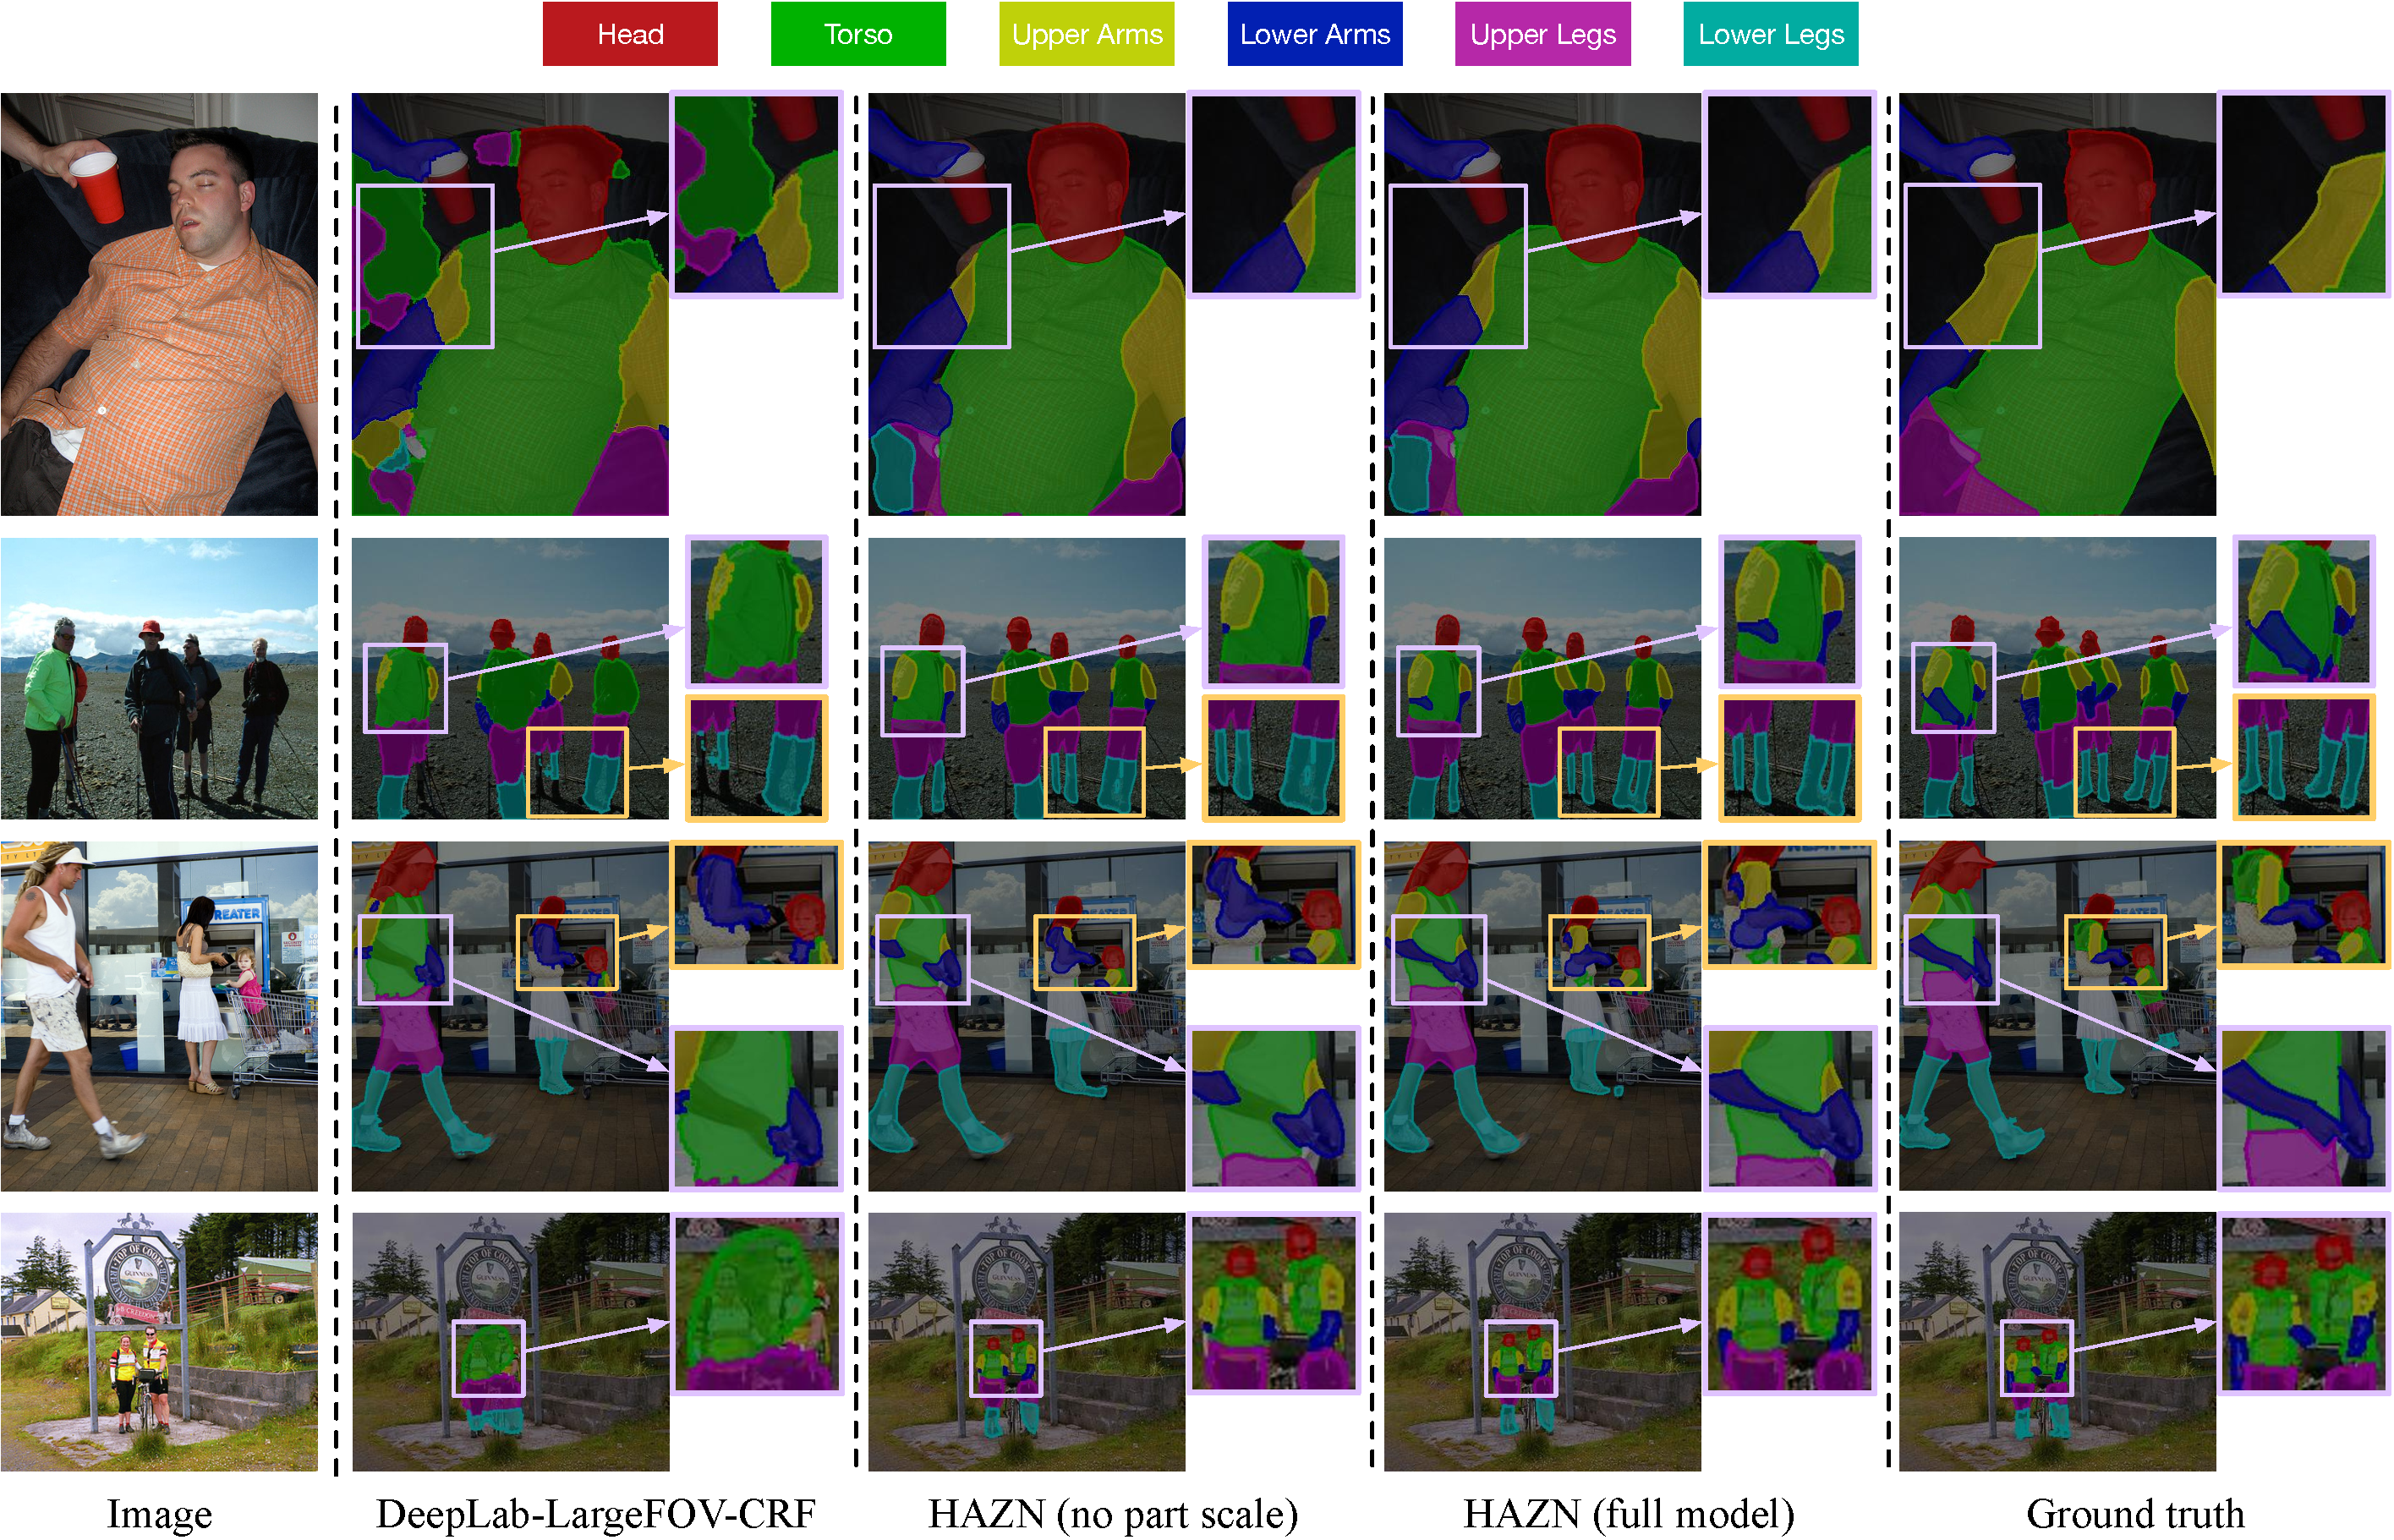
\includegraphics[width=1.00\linewidth]{figs/results_v3_eccv.pdf}
\caption{Qualitative comparison on the PASCAL-Person-Part dataset. We compare with DeepLab-LargeFOV-CRF~\cite{chen2016deeplab} and HAZN (no part scale). Our proposed HAZN models (the $3_{rd}$ and $4_{th}$ columns) attain better visual parsing results, especially for small scale human instances and small parts such as legs and arms.}
\label{fig:seg_image_eccv}
\end{figure*}

\paragraph{\textbf{Qualitative results.}} 
We visually show several example results from the PASCAL-Person-Part dataset in Fig.~\ref{fig:seg_image_eccv}. The baseline DeepLab-LargeFOV-CRF produces several errors due to lack of object and part scale information, e.g. background confusion ($1_{st}$ row), human part confusion ($3_{rd}$ row), or important part missing ($4_{th}$ row), yielding non-satisfactory part parsing results. Our HAZN (no part scale), which only contains object-scale AZN, already successfully relieves the confusions for large scale human instances while recovers the parts for small scale human instances. By further introducing part scale, the part details and boundaries are recovered even better, which are more visually satisfactory.

More visual examples are provided in Fig.~\ref{fig:human_res_eccv}, comparing with more baselines.
It can be seen that our full model (HAZN) gives much more satisfied part parsing results than the state-of-the-art baselines. Specifically, for small-scale human instances (e.g. the 1, 2, 5 rows of the figure), our HAZN recovers human parts like lower arms and lower legs and gives more accurate part boundaries; for medium-scale or large-scale human instances (e.g. the 3, 4, 9, 10 rows of the figure), our model relieves the local confusion with other parts or with the background.

\paragraph{\textbf{Failure cases.}}
Our typical failure modes are shown in Fig.~\ref{fig:seg_image_fail_eccv}. Compared with the baseline DeepLab-LargeFOV-CRF, our models give more reasonable parsing results with less local confusion, but they still suffer from heavy occlusion and unusual poses.

\begin{figure*}
\centering
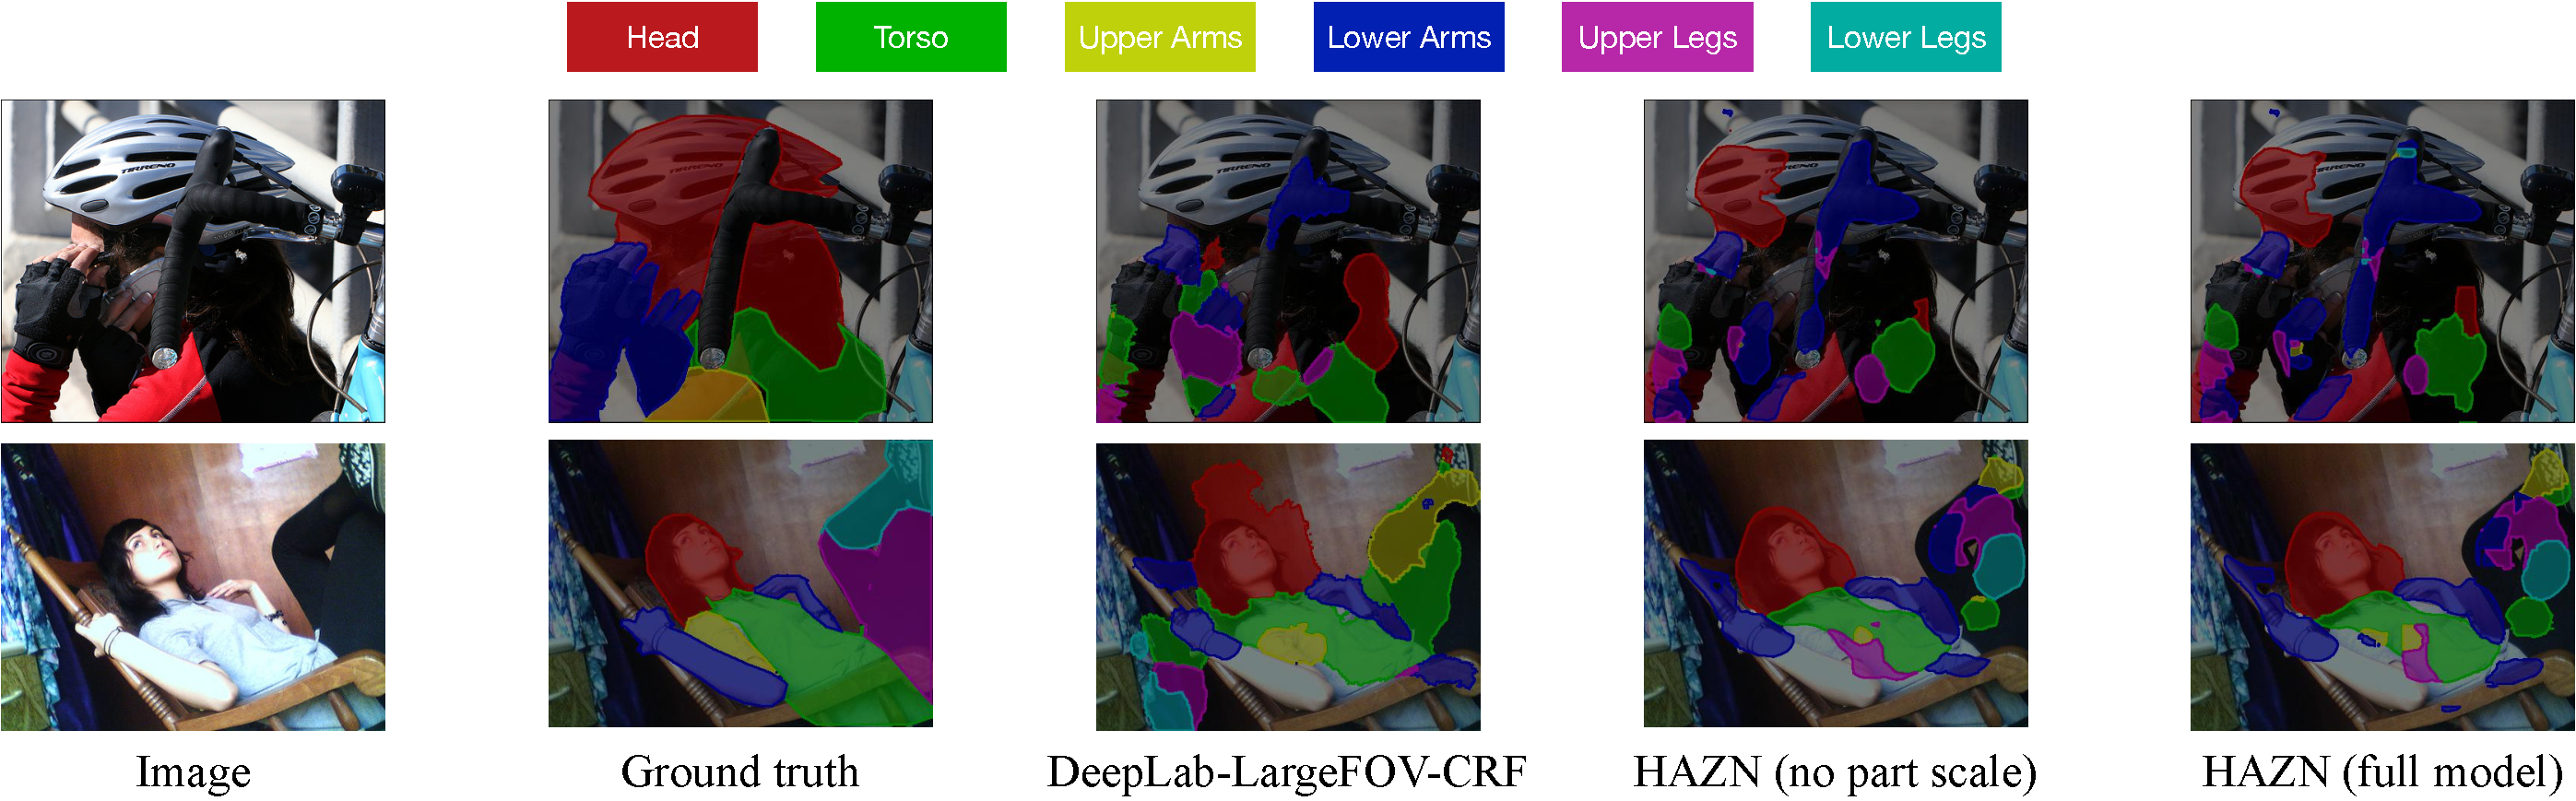
\includegraphics[width=1.0\linewidth]{figs/failure_modes_v2_eccv.pdf}
\caption{Failure cases for both the baseline and our models.}
\label{fig:seg_image_fail_eccv}
\end{figure*}

% More visual images.
\begin{figure*}
\centering
\hspace*{-0.4cm}
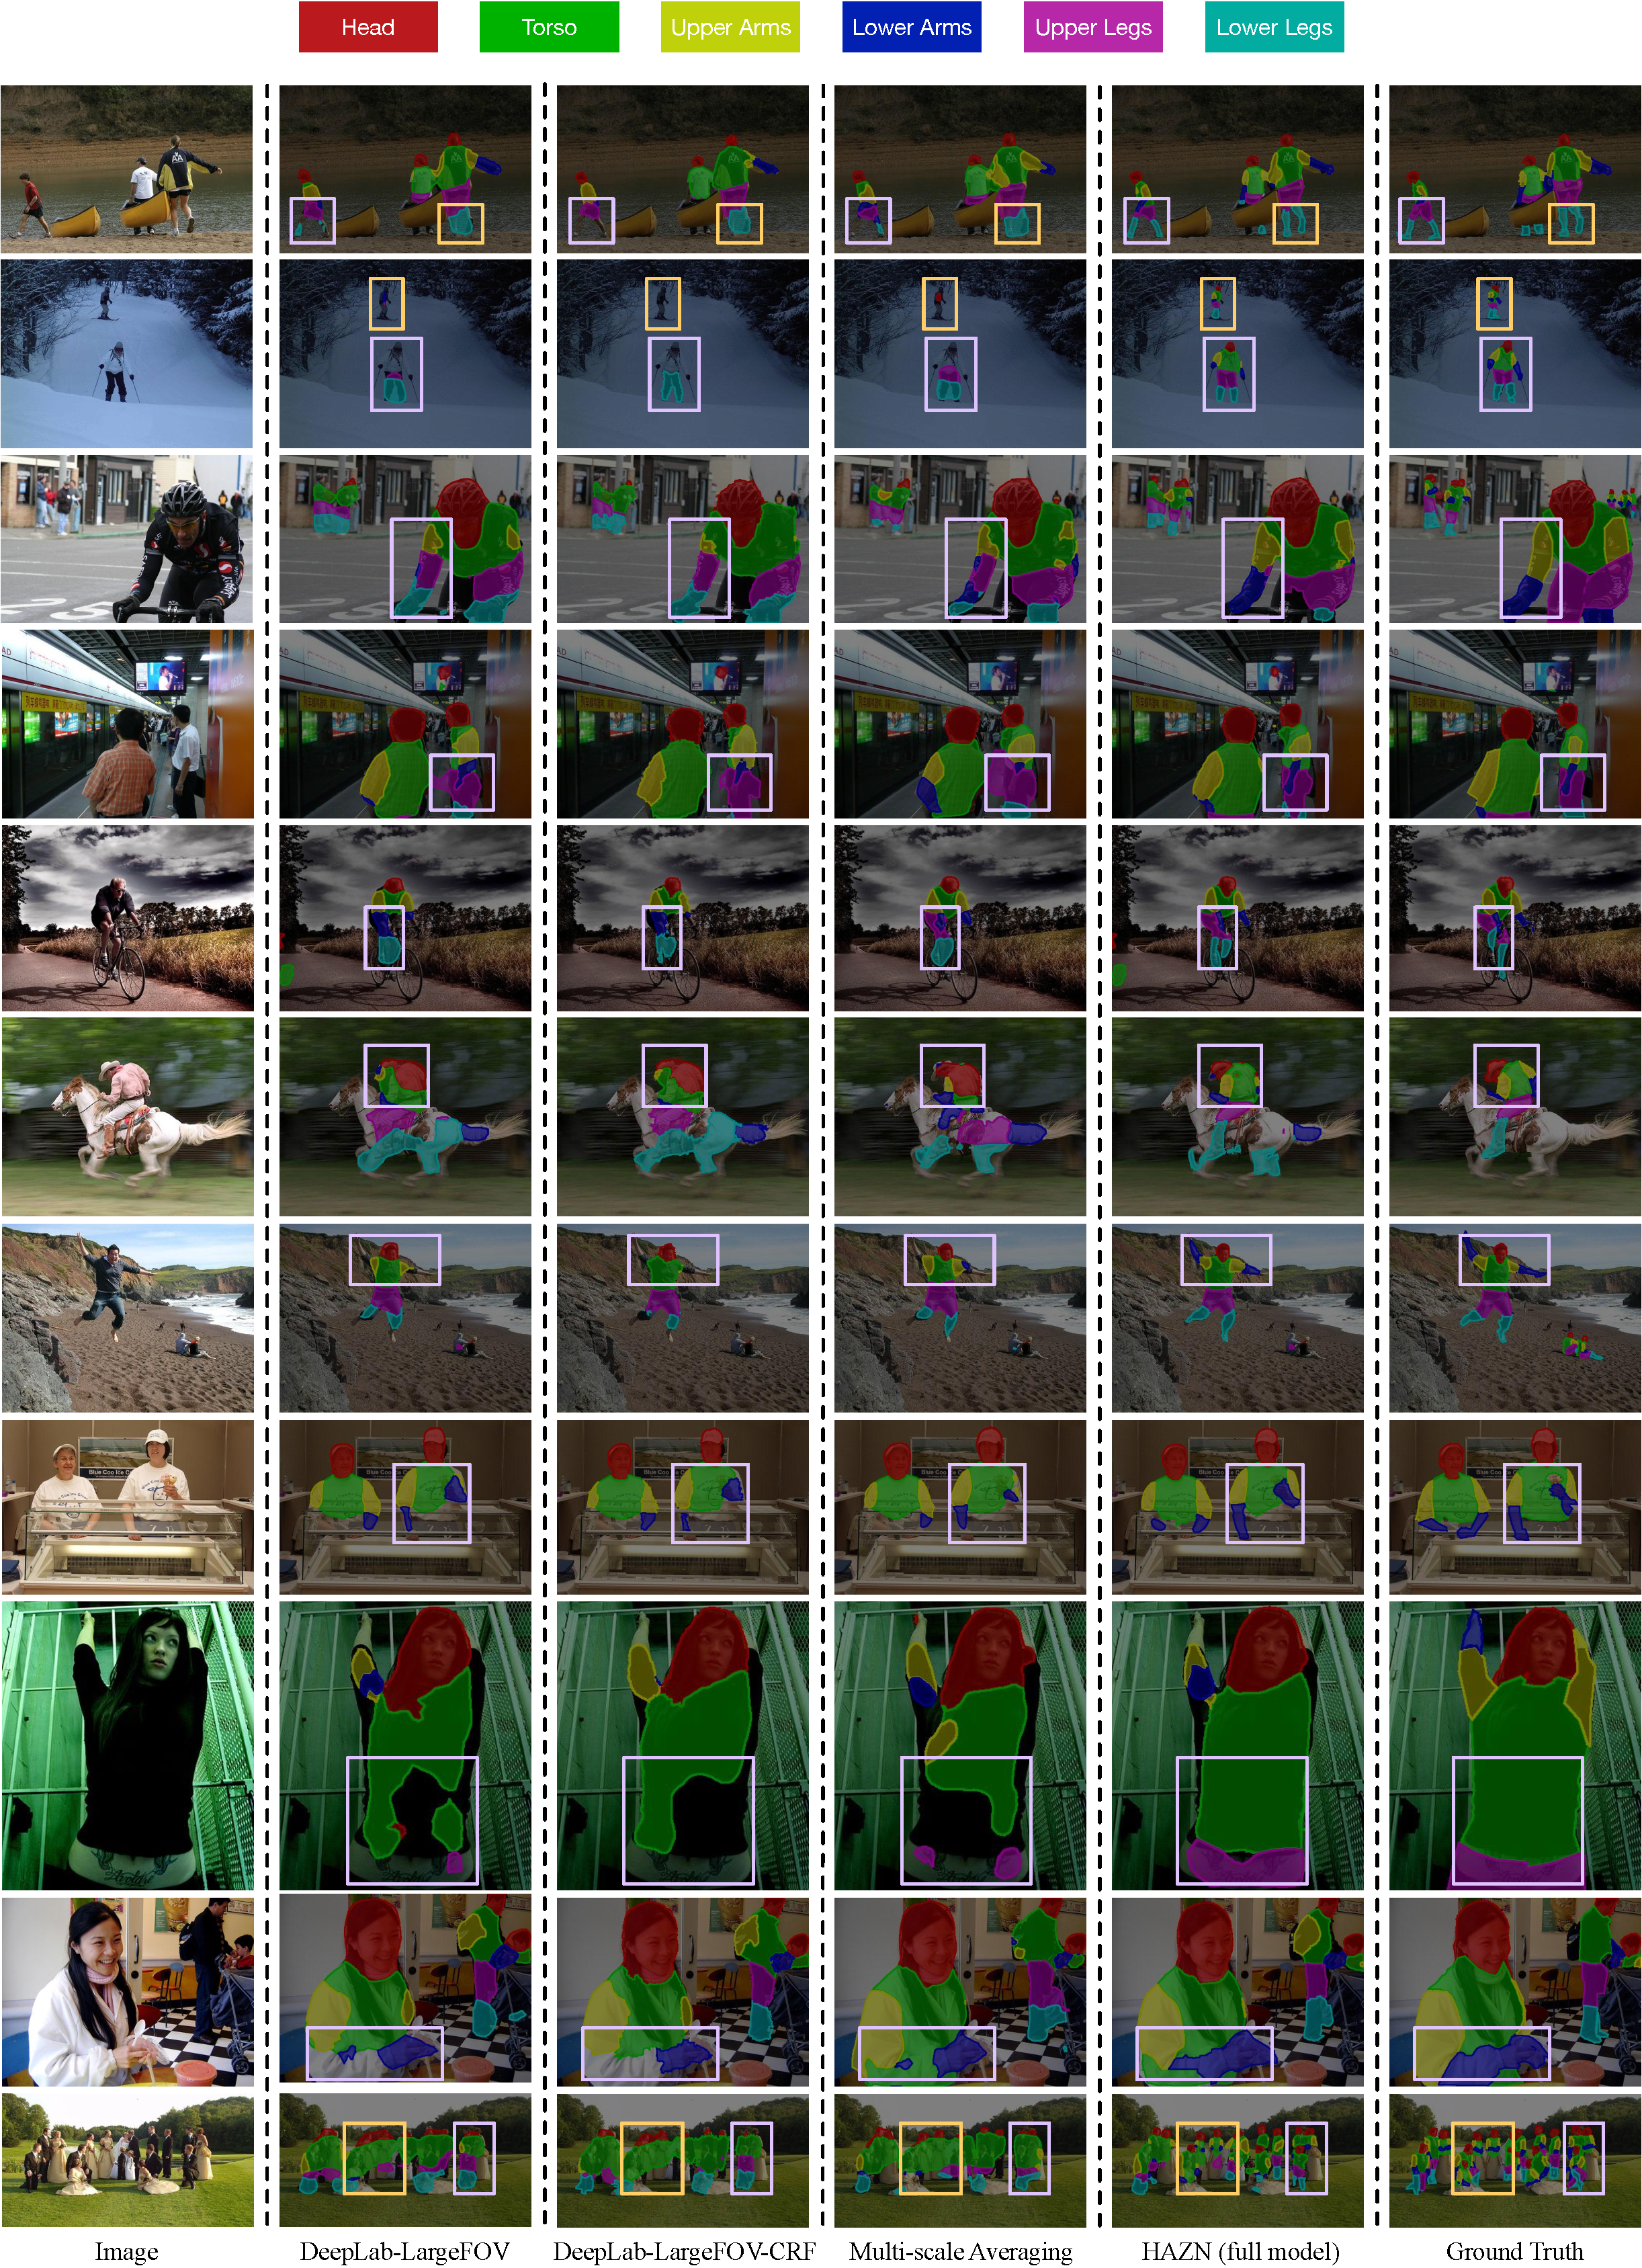
\includegraphics[width=0.95\linewidth]{figs/supplementary_results_eccv.pdf}
\vspace{-1\baselineskip}
\caption{More qualitative comparison on PASCAL-Person-Part. The baselines are explained in Sec.~\ref{subsubsec:human_parsing_eccv}.}
\label{fig:human_res_eccv}
\end{figure*}

\subsubsection{Experimental Results on the Horse-Cow Dataset}
\label{subsubsec:horses_eccv}
To show the generality of our HAZN approach to instance-wise object part segmentation,
we also applied our method to horse instances and cow instances presented in~\cite{wang2015semantic}.
All the testing procedures are the same as those described above for humans.

Copying the baseline numbers from~\cite{wang2015joint}, we give the part segmentation results for horses and cows in Tab.~\ref{table:seg_res_horse_cow_eccv}.
It shows that our baseline models from the DeepLab-LargeFOV~\cite{chen2016deeplab} already achieve competitive results
with the state-of-the-arts, while our HAZN provides a big improvement for horses and cows.
The improvement over the state-of-the-art JPO method~\cite{wang2015joint} is roughly 5\% mIOU.
It is most noticeable for small parts, e.g. the improvement for detecting horse/cow head and cow tails is more than 10$\%$.
This shows that our ``auto-zoom'' strategy can be effectively generalized to other objects for part segmentation.

\begin{table}
\centering
  \setlength{\tabcolsep}{5pt}
  \resizebox{0.9\columnwidth}{!}{
  \begin{tabular}{l |c c c c c | c}
	  \toprule[0.2 em]
	  \multicolumn{7}{c}{Horse} \\
	  \midrule
	  Method & Bkg & head & body & leg & tail &  Avg. \\ \midrule 
	  SPS & 79.14 & 47.64 & 69.74 & 38.85 & -  & - \\
	  HC$^*$ & 85.71 & 57.30 & 77.88 & 51.93 & 37.10  & 61.98 \\
	  JPO & {87.34} & {60.02} & 77.52 & {58.35} & \textbf{51.88}  & {67.02} \\
	  \midrule
	  LargeFOV & 87.44 & 64.45 & 80.70 & 54.61 & 44.03 & 66.25 \\
	  HAZN & \textbf{90.94}  & \textbf{70.75} &  \textbf{84.49}  & \textbf{63.91}  & 51.73 & \textbf{72.36} \\
	  \midrule [0.1 em]
	  \multicolumn{7}{c}{Cow} \\ \midrule
	  Method & Bkg & head & body & leg & tail &  Avg. \\ \midrule 
	  SPS & 78.00 & 40.55 & 61.65 & 36.32 & -  & - \\
	  HC$^*$ & 81.86 & 55.18 & 72.75 & 42.03 & 11.04 & 52.57 \\
	  JPO & {85.68} & {58.04} & {76.04} & {51.12} & {15.00} & {57.18} \\ \midrule
	  LargeFOV & 86.56 & 62.76 & 78.42 & 48.83 & 19.97 & 59.31 \\
	  HAZN & \textbf{90.71}  & \textbf{75.18}  &  \textbf{83.33}  & \textbf{57.42}  & \textbf{29.37}  &  \textbf{67.20} \\
	  \bottomrule[0.1 em]
  \end{tabular}
  }
 \caption{Part segmentation accuracy over the Horse-Cow dataset in terms of mean IOU (mIOU). We compare with the semantic part segmentation (SPS)~\cite{wang2015semantic}, the Hypercolumn (HC$^*$)~\cite{hariharan2015hypercolumns} and the joint part and object (JPO) results~\cite{wang2015joint}. We also list the performance of DeepLab-LargeFOV (LargeFOV)~\cite{chen2016deeplab}.}
 \label{table:seg_res_horse_cow_eccv}
\end{table}

We also provide qualitative evaluations in Fig.~\ref{fig:horse_cow_res_eccv}, comparing our full model with three state-of-the-art baselines. The three baselines are explained in Sec.~\ref{subsubsec:human_parsing_eccv}. We can observe that using our model, small parts such as legs and tails have been effectively recovered, and the boundary accuracy of all parts has been improved. 

% More visual images of horses and cows
\begin{figure*}
\centering
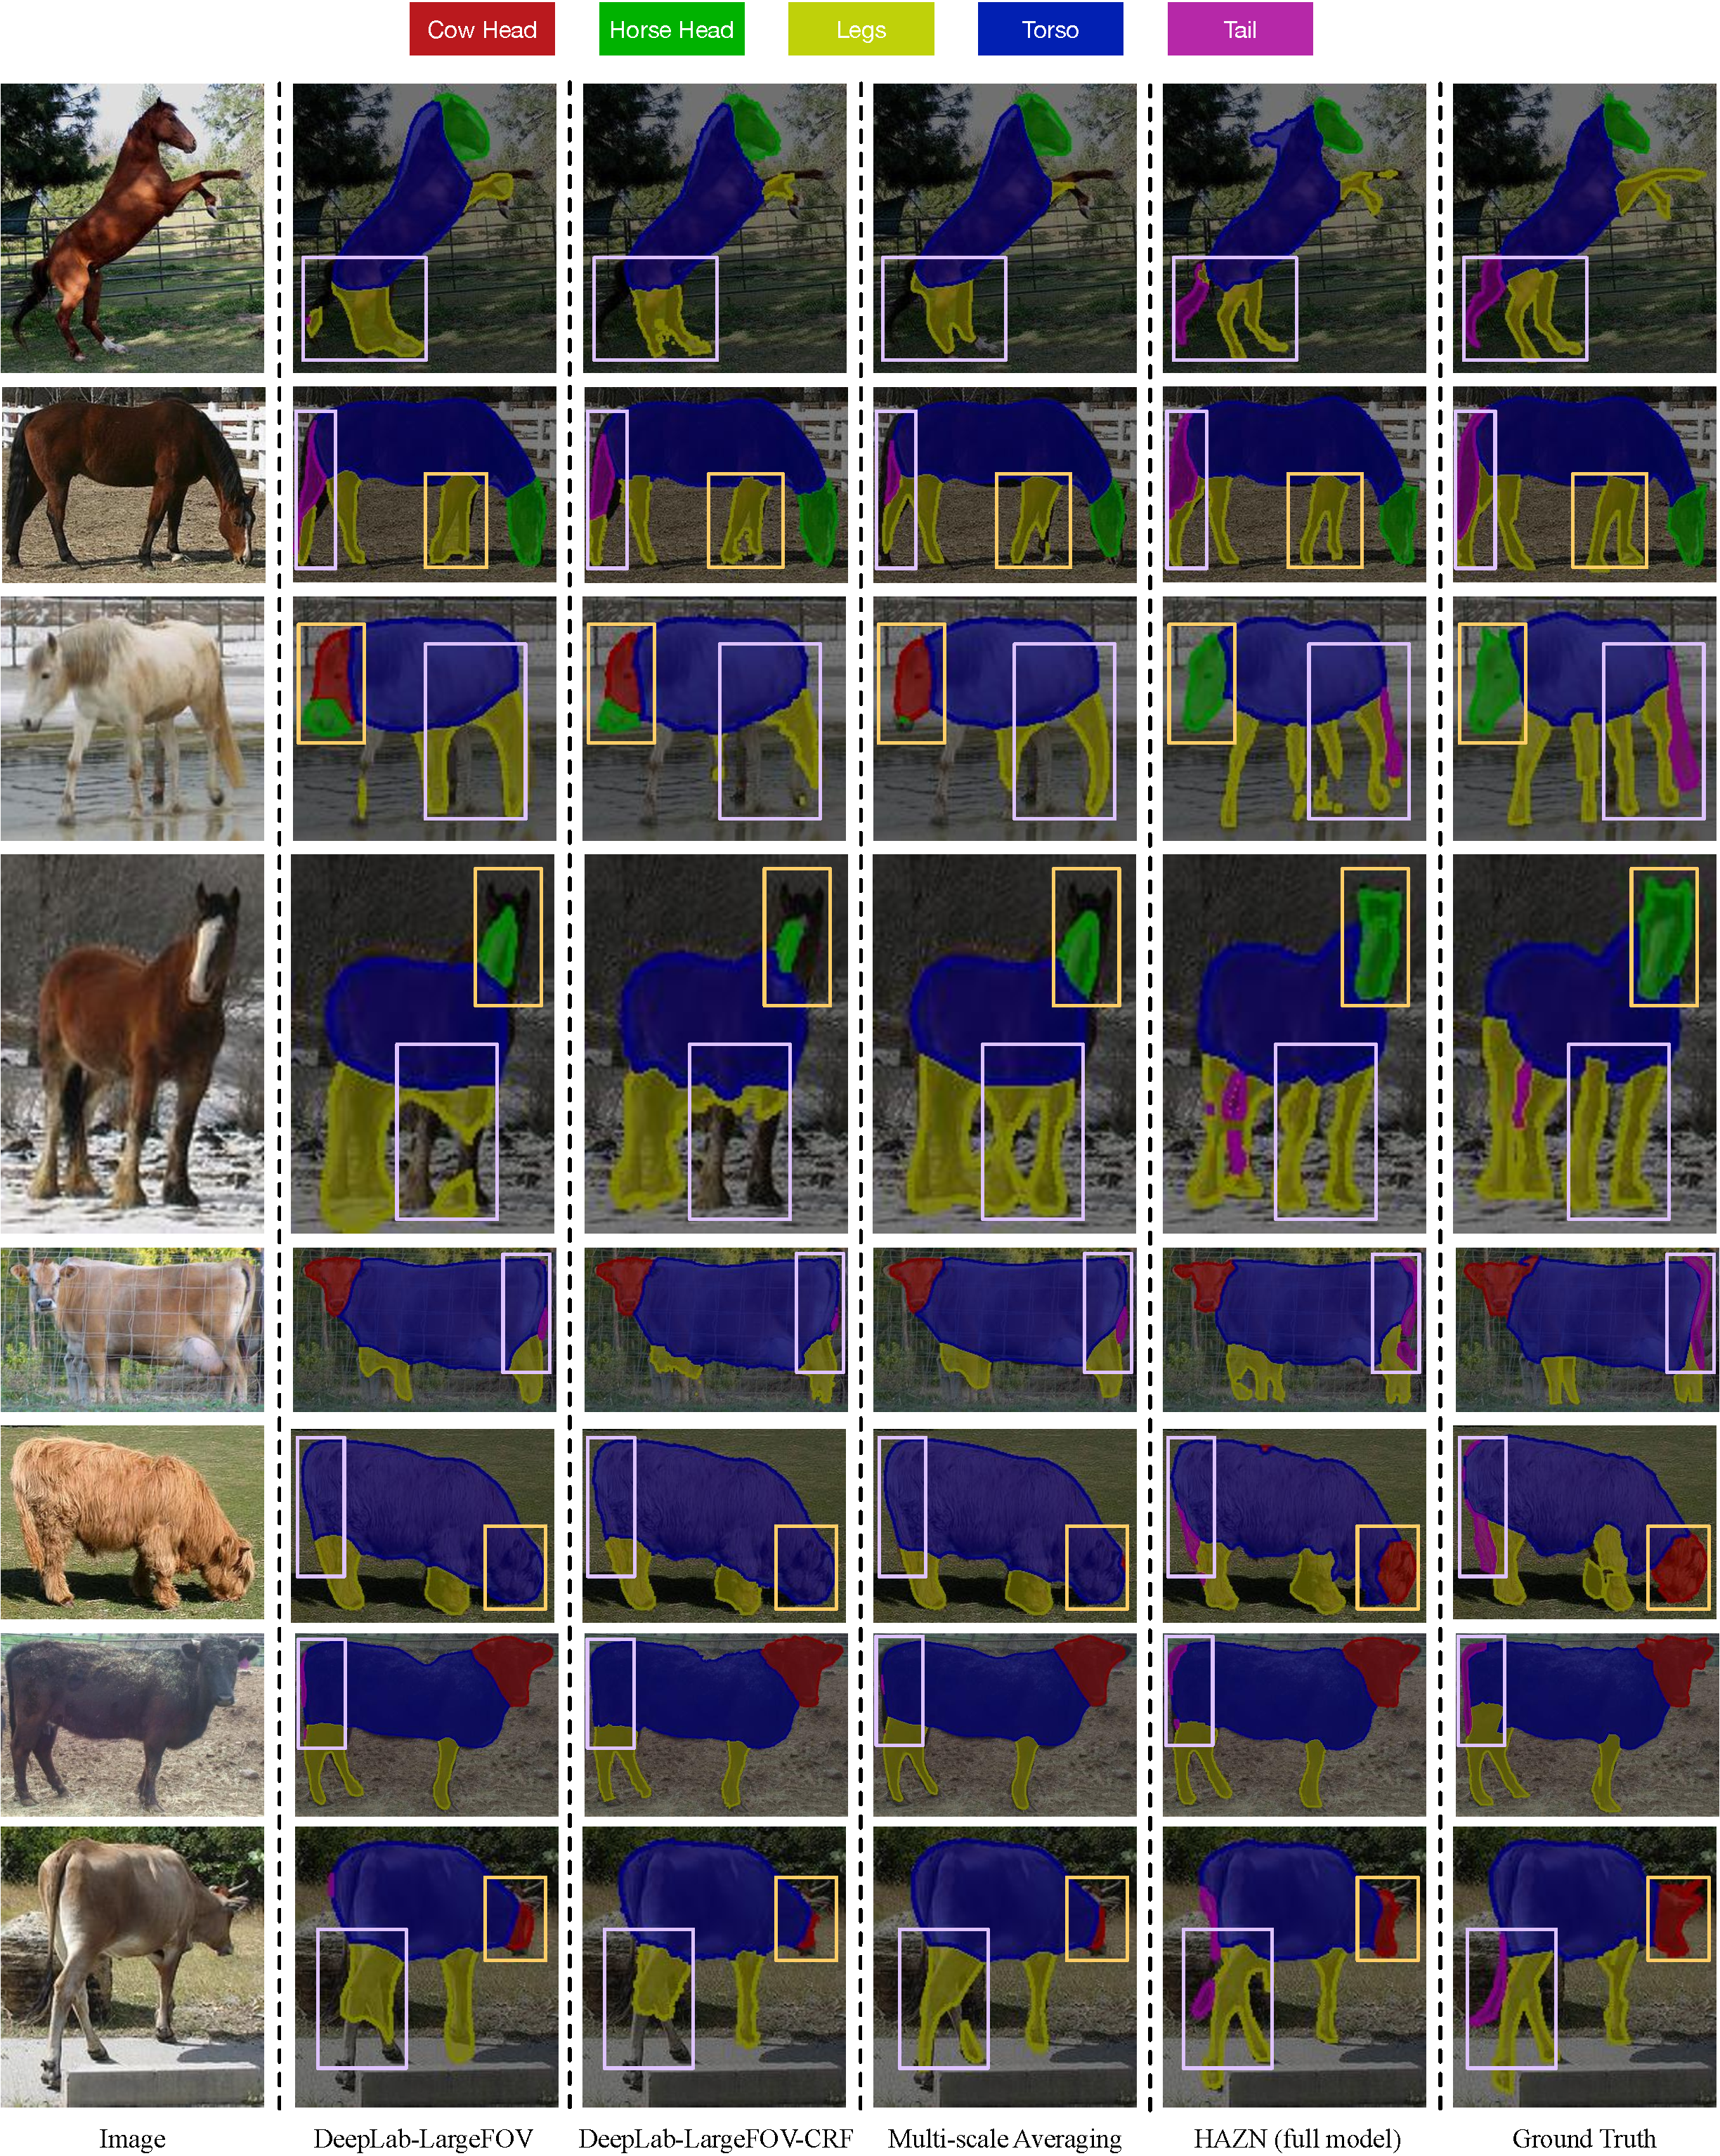
\includegraphics[width=0.95\linewidth]{figs/horse_cow_visual_results_eccv.pdf}
\caption{Qualitative comparison on the Horse-Cow Dataset. The baselines are explained in Sec.~\ref{subsubsec:human_parsing_eccv}.}
\label{fig:horse_cow_res_eccv}
\end{figure*}

\subsection{Summary}
To handle the big variation in natural images, we explain in this chapter an object part segmentation model called Hierarchical Auto-Zoom Net (HAZN), yieleding per-pixel segmentation of object parts. It adaptively estimates the scales of objects, and their parts, by a two-stage process of Auto-Zoom Nets. We perform extensive experiments on the challenging PASCAL dataset, showing that HAZN performs significantly better compared to state of the art methods, when applied to humans, horses and cows.

Unlike standard methods which process the image at a fixed range of scales, HAZN’s strategy of searching for objects and then for parts enables it, for example, to zoom in to small image regions and enlarge them to scales which would be prohibitively expensive (in terms of memory) if applied to the entire image (as fixed scale methods would require).

The ``auto-zoom'' idea of HAZN can be easily applied to other tasks, e.g. human pose estimation, fine-grained part localization, and so on.
In Sec.~\ref{sec:pose_and_seg}, we use the ``auto-zoom'' idea to significantly improve the performance of multi-person human pose estimation in
natural images.

Looking at the failure cases of HAZN (see Fig.~\ref{fig:seg_image_fail_eccv}), we notice that HAZN can still make errors about the overall pose configuration (e.g. labeling arms as legs, labeling a second person’s legs as the first person’s, etc.) when the person is in an extreme pose,
or the appearance of different parts are very similar, or there are other people overlapping with this person.
This motivates us to combine useful top-down pose information with the deep-based segmentation model HAZN, which we also explore in Sec.~\ref{sec:pose_and_seg}.

\section{Joint Prediction of Pose Estimation and Semantic Part Segmentation}
\label{sec:pose_and_seg}
Human pose estimation and semantic part segmentation are two crucial and correlated tasks in human-centric analysis. However, the two tasks are mostly solved independently without considering their correlations.
In fact, the two tasks are complementary and solving them jointly can reduce the learning difficulty of addressing each of them individually. As demonstrated in the middle column of Fig.~\ref{fig:motivation_cvpr}, for pose estimation, using loss functions w.r.t. the joints solely may omit the knowledge of pixel-wise part appearance coherence, yielding joints located outside a human instance or misleading joints when two people are close to each other; for part segmentation, on the other hand, using a loss function that only respects pixel-wise part labels tends to lack the proper overall human shape regularization, yielding missing or errorneous predictions when the appearance cues are weak or missing. As shown in the right column of Fig.~\ref{fig:motivation_cvpr}, by handling pose estimation and semantic part segmentation jointly, the ambiguity in pose estimation (e.g. out of instance region) can be corrected by considering semantic part segments, while the estimated pose skeleton provides object-level context and regularity to help part segments align with human instances, e.g. over the details of arms and legs where appearance cues are missing.

In Sec.~\ref{sec:hazn}, we introduce a deep-based part segmentation model, Hierarchical Auto-Zoom Net (HAZN), which performs quite well on the challenging dataset PASCAL. However, we notice that some severe pose errors can't be avoided and the boundary details of arms and legs are not satisfactory.
This motivates us to propose a ``pose-guided'' semantic part segmentation model, which incorporates top-down pose cues into HAZN, performing pose estimation and semantic part segmentation jointly.

Specifically, we illustrate the framework of the joint prediction model in Fig.~\ref{fig:framework_cvpr}.
Firstly, given an image that contains multiple people, we train two FCNs: Pose FCN and Part FCN.
Similar to~\cite{insafutdinov2016deepercut}, the Pose FCN outputs the pixel-wise joint score map,
i.e. the potential of joints at each pixel (how likely a type of joint is located at certain pixel),
and also outputs the joint neighbour score map, i.e. the potential of the location likelihood of neighboring joints for each joint type.
The Part FCN produces the part score map for each semantic part type.
Secondly, the three types of information are fused through a FCRF to refine the human joint locations, where a novel smoothness term on both part segments and joint proposals (generated from the initially estimated pixel-wise joint score map) are applied to encourage the consistency between segments and joints.
Thirdly, the refined pose joints are re-organized into pose features that encode overall shape information, and are fed into a second-stage Part FCN as an additional input besides the initial part score map, yielding better segmentation results.
To reduce the complexity of the FCRF, rather than infer over the full image as~\cite{insafutdinov2016deepercut}, we adopt a human detector~\cite{ren2015faster} to first get the bounding box for each human instance and resize each instance region using the ``auto-zoom'' idea described in Sec.~\ref{sec:hazn}.
Our whole inference procedure is then performed within each resized region.

In order to train and evaluate the joint prediction model, we augment the challenging PASCAL-Person-Part dataset~\cite{chen2014detect} with 14 human pose joint locations through manual labeling and make the annotations public. This dataset includes 3533 images that contain large variation of human poses, scales and occlusion. We evaluate our method over this dataset, and show that our approach outperforms the most recent competing methods for both tasks. In particular, our method is more effective and much faster (8 seconds versus 4 minutes) than DeeperCut~\cite{insafutdinov2016deepercut} which is arguably the most effective algorithm for multi-person pose estimation.

\begin{figure*}[!tb]
\begin{center}
   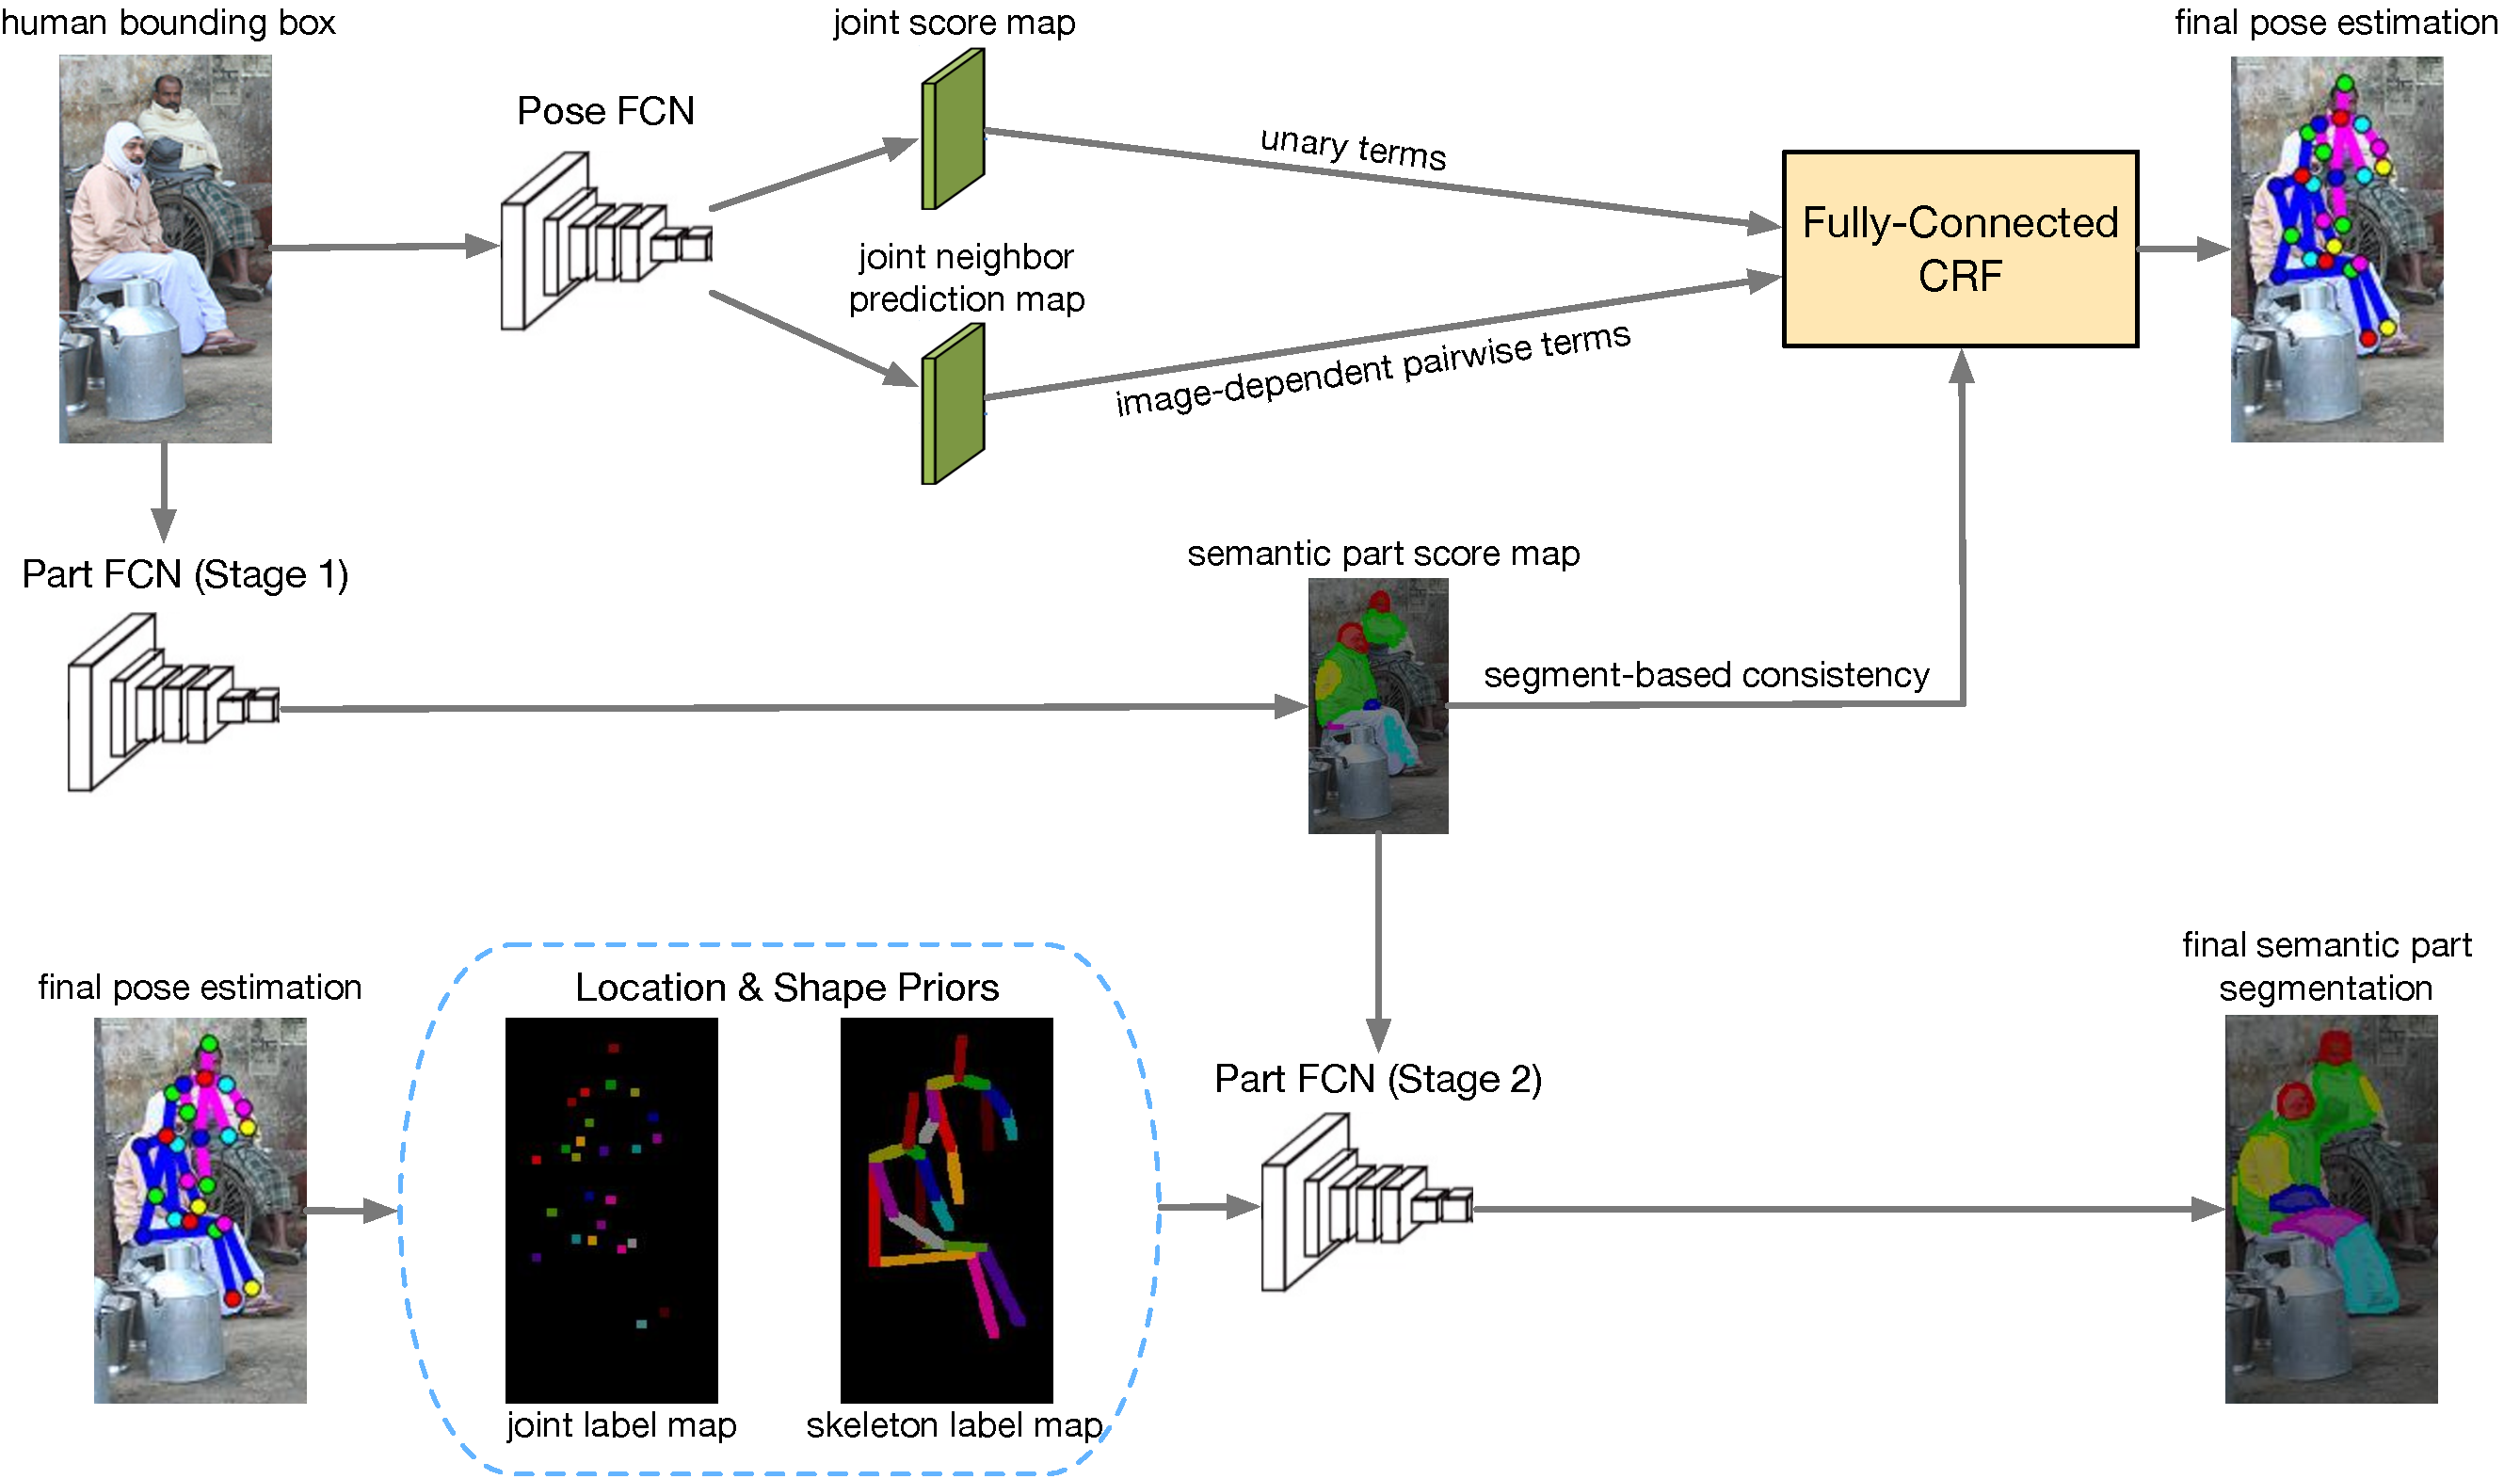
\includegraphics[width=0.95\textwidth]{figs/framework_v2_cvpr.pdf}
\end{center}
\caption{The framework of our joint pose estimation and part segmentation model. Initial joint scores and part segment scores are fused to yield better pose estimation results, and then the estimated poses are used to refine part segmentation.}
\label{fig:framework_cvpr}
\end{figure*}

\subsection{The Model}

\subsection{Experiments}

\subsection{Summary}

\section{Conclusion}

\begin{acknowledgements}
AAA
\end{acknowledgements}

% BibTeX users please use one of
%\bibliographystyle{spbasic}      % basic style, author-year citations
%\bibliographystyle{spmpsci}      % mathematics and physical sciences
%\bibliographystyle{spphys}       % APS-like style for physics
%\bibliography{ijcv.bib}   % name your BibTeX data base

\begin{thebibliography}{}
%
% and use \bibitem to create references. Consult the Instructions
% for authors for reference list style.
%
%\bibitem{RefJ}
% Format for Journal Reference
%Author, Article title, Journal, Volume, page numbers (year)
% Format for books
%\bibitem{RefB}
%Author, Book title, page numbers. Publisher, place (year)
%
% Semantic part segmentation
\bibitem{rauschert2012generative}
Rauschert, Ingmar, and Robert T. Collins. "A generative model for simultaneous estimation of human body shape and pixel-level segmentation." In European Conference on Computer Vision, pp. 704-717 (2012)
\bibitem{long2015fully}
Long, Jonathan, Evan Shelhamer, and Trevor Darrell. "Fully convolutional networks for semantic segmentation." In Proceedings of the IEEE Conference on Computer Vision and Pattern Recognition (CVPR), pp. 3431-3440 (2015)
\bibitem{wang2015joint}
Wang, Peng, Xiaohui Shen, Zhe Lin, Scott Cohen, Brian Price, and Alan L. Yuille. "Joint object and part segmentation using deep learned potentials." In Proceedings of the IEEE International Conference on Computer Vision, pp. 1573-1581 (2015)
\bibitem{chen2016deeplab}
Chen, Liang-Chieh, George Papandreou, Iasonas Kokkinos, Kevin Murphy, and Alan L. Yuille. "Deeplab: Semantic image segmentation with deep convolutional nets, atrous convolution, and fully connected crfs." arXiv preprint arXiv:1606.00915 (2016)
\bibitem{bo2011shape}
Bo, Yihang, and Charless C. Fowlkes. "Shape-based pedestrian parsing." In Proceedings of the IEEE Conference on Computer Vision and Pattern Recognition (CVPR), pp. 2265-2272 (2011)
\bibitem{eslami2012generative}
Eslami, S., and Christopher Williams. "A generative model for parts-based object segmentation." In Advances in Neural Information Processing Systems (NIPS), pp. 100-107 (2012)
\bibitem{yamaguchi2012parsing}
Yamaguchi, Kota, M. Hadi Kiapour, Luis E. Ortiz, and Tamara L. Berg. "Parsing clothing in fashion photographs." In Proceedings of the IEEE Conference on Computer Vision and Pattern Recognition (CVPR), pp. 3570-3577 (2012)
\bibitem{dong2013deformable}
Dong, Jian, Qiang Chen, Wei Xia, Zhongyang Huang, and Shuicheng Yan. "A deformable mixture parsing model with parselets." In International Conference on Computer Vision (ICCV), pp. 3408-3415 (2013)
\bibitem{zhu2011max}
Zhu, Long Leo, Yuanhao Chen, Chenxi Lin, and Alan Yuille. "Max margin learning of hierarchical configural deformable templates (hcdts) for efficient object parsing and pose estimation." In International Journal of Computer Vision, 93(1), pp 1-21 (2011)
\bibitem{hariharan2015hypercolumns}
Hariharan, Bharath, Pablo Arbeláez, Ross Girshick, and Jitendra Malik. "Hypercolumns for object segmentation and fine-grained localization." In Proceedings of the IEEE Conference on Computer Vision and Pattern Recognition (CVPR), pp. 447-456 (2015)
\bibitem{krahenbuhl2011efficient}
Krähenbühl, Philipp, and Vladlen Koltun. "Efficient inference in fully connected crfs with gaussian edge potentials." In Advances in Neural Information Processing Systems (NIPS), pp. 109-117 (2011)
\bibitem{xia2016pose}
Xia, Fangting, Jun Zhu, Peng Wang, and Alan L. Yuille. "Pose-Guided Human Parsing by an AND/OR Graph Using Pose-Context Features." In AAAI, pp. 3632-3640 (2016)
\bibitem{chen2016attention}
Chen, Liang-Chieh, Yi Yang, Jiang Wang, Wei Xu, and Alan L. Yuille. "Attention to scale: Scale-aware semantic image segmentation." In Proceedings of the IEEE conference on Computer Vision and Pattern Recognition (CVPR), pp. 3640-3649 (2016)
\bibitem{ladicky2013human}
Ladicky, Lubor, Philip HS Torr, and Andrew Zisserman. "Human pose estimation using a joint pixel-wise and part-wise formulation." In proceedings of the IEEE Conference on Computer Vision and Pattern Recognition (CVPR), pp. 3578-3585 (2013)
\bibitem{dong2014towards}
Dong, Jian, Qiang Chen, Xiaohui Shen, Jianchao Yang, and Shuicheng Yan. "Towards unified human parsing and pose estimation." In proceedings of the IEEE Conference on Computer Vision and Pattern Recognition (CVPR), pp. 843-850 (2014)
\bibitem{wang2015semantic}
Wang, Jianyu, and Alan L. Yuille. "Semantic part segmentation using compositional model combining shape and appearance." In Proceedings of the IEEE Conference on Computer Vision and Pattern Recognition (CVPR), pp. 1788-1797 (2015)
%
% semantic object segmentation
\bibitem{dai2015boxsup}
Dai, Jifeng, Kaiming He, and Jian Sun. "Boxsup: Exploiting bounding boxes to supervise convolutional networks for semantic segmentation." In Proceedings of the IEEE International Conference on Computer Vision (ICCV), pp. 1635-1643 (2015)
\bibitem{papandreou2015weakly}
Papandreou, George, Liang-Chieh Chen, Kevin Murphy, and Alan L. Yuille. "Weakly-and semi-supervised learning of a DCNN for semantic image segmentation." arXiv preprint arXiv:1502.02734 (2015)
%
% Pose estimation
\bibitem{yang2011articulated}
Yang, Yi, and Deva Ramanan. "Articulated pose estimation with flexible mixtures-of-parts." In Proceedings of the IEEE Conference on Computer Vision and Pattern Recognition (CVPR), pp. 1385-1392 (2011).
\bibitem{tompson2015efficient}
Tompson, Jonathan, Ross Goroshin, Arjun Jain, Yann LeCun, and Christoph Bregler. "Efficient object localization using convolutional networks." In Proceedings of the IEEE Conference on Computer Vision and Pattern Recognition (CVPR), pp. 648-656 (2015)
\bibitem{chen2015parsing}
Chen, Xianjie, and Alan Yuille. "Parsing occluded people by flexible compositions." In Proceedings of the IEEE Conference on Computer Vision and Pattern Recognition (CVPR), pp. 3945-3954 (2015)
\bibitem{fischler1973representation}
Fischler, Martin A., and Robert A. Elschlager. "The representation and matching of pictorial structures." In IEEE Transactions on Computers, 100(1), pp. 67-92 (1973)
\bibitem{felzenszwalb2005pictorial}
Felzenszwalb, Pedro F., and Daniel P. Huttenlocher. "Pictorial structures for object recognition." In International Journal of Computer Vision, 61(1), pp. 55-79 (2005)
\bibitem{andriluka2009pictorial}
Andriluka, Mykhaylo, Stefan Roth, and Bernt Schiele. "Pictorial structures revisited: People detection and articulated pose estimation." In Proceedings of the IEEE Conference on Computer Vision and Pattern Recognition (CVPR), pp. 1014-1021 (2009)
\bibitem{sapp2013modec}
Sapp, Ben, and Ben Taskar. "Modec: Multimodal decomposable models for human pose estimation." In Proceedings of the IEEE Conference on Computer Vision and Pattern Recognition (CVPR), pp. 3674-3681 (2013)
\bibitem{zhu2008max}
Zhu, Long, Yuanhao Chen, Yifei Lu, Chenxi Lin, and Alan Yuille. "Max margin and/or graph learning for parsing the human body." In Proceedings of the IEEE Conference on Computer Vision and Pattern Recognition (CVPR), pp. 1-8 (2008)
\bibitem{rothrock2013integrating}
Rothrock, Brandon, Seyoung Park, and Song-Chun Zhu. "Integrating grammar and segmentation for human pose estimation." In Proceedings of the IEEE Conference on Computer Vision and Pattern Recognition (CVPR), pp. 3214-3221 (2013)
\bibitem{chen2014articulated}
Chen, Xianjie, and Alan L. Yuille. "Articulated pose estimation by a graphical model with image dependent pairwise relations." In Advances in Neural Information Processing Systems (NIPS), pp. 1736-1744 (2014)
\bibitem{toshev2014deeppose}
Toshev, Alexander, and Christian Szegedy. "Deeppose: Human pose estimation via deep neural networks." In Proceedings of the IEEE Conference on Computer Vision and Pattern Recognition (CVPR), pp. 1653-1660 (2014)
\bibitem{carreira2016human}
Carreira, Joao, Pulkit Agrawal, Katerina Fragkiadaki, and Jitendra Malik. "Human pose estimation with iterative error feedback." In Proceedings of the IEEE Conference on Computer Vision and Pattern Recognition (CVPR), pp. 4733-4742 (2016)
\bibitem{chu2016structured}
Chu, Xiao, Wanli Ouyang, Hongsheng Li, and Xiaogang Wang. "Structured feature learning for pose estimation." In Proceedings of the IEEE Conference on Computer Vision and Pattern Recognition (CVPR), pp. 4715-4723 (2016)
\bibitem{insafutdinov2016deepercut}
Insafutdinov, Eldar, Leonid Pishchulin, Bjoern Andres, Mykhaylo Andriluka, and Bernt Schiele. "Deepercut: A deeper, stronger, and faster multi-person pose estimation model." In European Conference on Computer Vision (ECCV), pp. 34-50 (2016)
%
% Fine-grained recognition
\bibitem{branson2014bird}
Branson, Steve, Grant Van Horn, Serge Belongie, and Pietro Perona. "Bird species categorization using pose normalized deep convolutional nets." arXiv preprint arXiv:1406.2952 (2014)
\bibitem{zhang2014part}
Zhang, Ning, Jeff Donahue, Ross Girshick, and Trevor Darrell. "Part-based R-CNNs for fine-grained category detection." In European Conference on Computer Vision, pp. 834-849 (2014)
\bibitem{krause2016unreasonable}
Krause, Jonathan, Benjamin Sapp, Andrew Howard, Howard Zhou, Alexander Toshev, Tom Duerig, James Philbin, and Li Fei-Fei. "The unreasonable effectiveness of noisy data for fine-grained recognition." In European Conference on Computer Vision, pp. 301-320 (2016)
%
% Action recognition
\bibitem{wang2012discriminative}
Wang, Yang, Duan Tran, Zicheng Liao, and David Forsyth. "Discriminative hierarchical part-based models for human parsing and action recognition." In Journal of Machine Learning Research, 13(Oct), pp. 3075-3102 (2012)
\bibitem{zhou2015interaction}
Zhou, Yang, Bingbing Ni, Richang Hong, Meng Wang, and Qi Tian. "Interaction part mining: A mid-level approach for fine-grained action recognition." In Proceedings of the IEEE Conference on Computer Vision and Pattern Recognition (CVPR), pp. 3323-3331 (2015)
\bibitem{chunyu_action}
Wang, Chunyu, Yizhou Wang, and Alan L. Yuille. "An approach to pose-based action recognition." In Proceedings of the IEEE Conference on Computer Vision and Pattern Recognition (CVPR), pp. 915-922 (2013)
%
% Person identification
\bibitem{ma2011human}
Ma, Lianyang, Xiaokang Yang, Yi Xu, and Jun Zhu. "Human identification using body prior and generalized EMD." In Image Processing (ICIP) 18th IEEE International Conference, pp. 1441-1444 (2011)
\bibitem{zhao2017deeply}
Zhao, Liming, Xi Li, Jingdong Wang, and Yueting Zhuang. "Deeply-learned part-aligned representations for person re-identification." arXiv preprint arXiv:1707.07256 (2017)
%
% Video surveillance
\bibitem{gallego2008segmentation}
Gallego, Jaime, Montse Pardas, and Jose-Luis Landabaso. "Segmentation and tracking of static and moving objects in video surveillance scenarios." In Image Processing (ICIP) 15th IEEE International Conference, pp. 2716-2719 (2008)
\bibitem{liu2017surveillance}
Liu, Si, Changhu Wang, Ruihe Qian, Han Yu, Renda Bao, and Yao Sun. "Surveillance video parsing with single frame supervision." In IEEE Conference on Computer Vision and Pattern Recognition (CVPR) workshops, pp. 1-9 (2017)
% 
% Object Detection
\bibitem{huang2015densebox}
Huang, Lichao, Yi Yang, Yafeng Deng, and Yinan Yu. "Densebox: Unifying landmark localization with end to end object detection." arXiv preprint arXiv:1509.04874 (2015)
\bibitem{liang2015proposal}
Liang, Xiaodan, Yunchao Wei, Xiaohui Shen, Jianchao Yang, Liang Lin, and Shuicheng Yan. "Proposal-free network for instance-level object segmentation." arXiv preprint arXiv:1509.02636 (2015)
\bibitem{ren2015faster}
Ren, Shaoqing, Kaiming He, Ross Girshick, and Jian Sun. "Faster r-cnn: Towards real-time object detection with region proposal networks." In Advances in Neural Information Processing Systems (NIPS), pp. 91-99 (2015)
\bibitem{redmon2016you}
Redmon, Joseph, Santosh Divvala, Ross Girshick, and Ali Farhadi. "You only look once: Unified, real-time object detection." In Proceedings of the IEEE Conference on Computer Vision and Pattern Recognition (CVPR), pp. 779-788 (2016)
%
% Dataset
\bibitem{chen2014detect}
Chen, Xianjie, Roozbeh Mottaghi, Xiaobai Liu, Sanja Fidler, Raquel Urtasun, and Alan Yuille. "Detect what you can: Detecting and representing objects using holistic models and body parts." In Proceedings of the IEEE Conference on Computer Vision and Pattern Recognition (CVPR), pp. 1971-1978 (2014)
%
% Background
\bibitem{dalal2005histograms}
Dalal, Navneet, and Bill Triggs. "Histograms of oriented gradients for human detection." In Proceedings of the IEEE Conference on Computer Vision and Pattern Recognition (CVPR), pp. 886-893 (2005)
\bibitem{belongie2001shape}
Belongie, Serge, Jitendra Malik, and Jan Puzicha. "Shape context: A new descriptor for shape matching and object recognition." In Advances in Neural Information Processing Systems (NIPS), pp. 831-837 (2001)
\bibitem{everingham2014pascal}
Everingham, Mark, SM Ali Eslami, Luc Van Gool, Christopher KI Williams, John Winn, and Andrew Zisserman. "The pascal visual object classes challenge: A retrospective." In International Journal of Computer Vision 111, no. 1, pp 98-136 (2015)
\bibitem{li2014secrets}
Li, Yin, Xiaodi Hou, Christof Koch, James M. Rehg, and Alan L. Yuille. "The secrets of salient object segmentation." In Proceedings of the IEEE Conference on Computer Vision and Pattern Recognition (CVPR), pp. 280–287 (2014)
%
% Related works
\bibitem{arbelaez2009contours}
Arbelaez, Pablo, Michael Maire, Charless Fowlkes, and Jitendra Malik. "From contours to regions: An empirical evaluation." In Proceedings of the IEEE Conference on Computer Vision and Pattern Recognition (CVPR), pp. 2294-2301 (2009)
\bibitem{carreira2012cpmc}
Carreira, Joao, and Cristian Sminchisescu. "Cpmc: Automatic object segmentation using constrained parametric min-cuts." In IEEE Transactions on Pattern Analysis and Machine Intelligence, 34(7), pp 1312-1328 (2012)
\bibitem{girshick2014rich}
Girshick, Ross, Jeff Donahue, Trevor Darrell, and Jitendra Malik. "Rich feature hierarchies for accurate object detection and semantic segmentation." In Proceedings of the IEEE conference on Computer Vision and Pattern Recognition (CVPR), pp. 580-587 (2014)
\bibitem{lecun1998gradient}
LeCun, Yann, Léon Bottou, Yoshua Bengio, and Patrick Haffner. "Gradient-based learning applied to document recognition." In Proceedings of the IEEE, 86(11), pp. 2278-2324 (1998)

\end{thebibliography}

\end{document}
% end of file template.tex

